%%%%%%%%%%%%%%%%%%%%%%%%%%%%%%%%%%%%%%%%%%%%%%%%%%%%%%%%%%%%%%%%%%%%%%
% Lớp 11 | Giới hạn. Hàm số liên tục | Giới hạn của hàm số
% Dạng 1D3?2-7: Giới hạn một bên
% Số câu: 82  (sinh tự động bởi tach_cau.py; từ nay thầy sửa trực tiếp file này)
%%%%%%%%%%%%%%%%%%%%%%%%%%%%%%%%%%%%%%%%%%%%%%%%%%%%%%%%%%%%%%%%%%%%%%

%%%%%%%%%%%%%%%% TRẮC NGHIỆM 4 PHƯƠNG ÁN %%%%%%%%%%%%%%%%

% nguồn: Ok_Toan11_TracNghiem_Lan2
\begin{ex}%[1D3N2-7]%[ma:473e390a]
	Tính  giới hạn $L=\lim\limits_{x\to-1}\dfrac{x^2-x-2+1}{3x^2+8x+5}$.
	\choice 
		{\True$L=-\dfrac{3}{2}$} 
		 {$L=\dfrac{1}{2}$}
		{$L=-\infty$} 
		 {$L=0$}
	\loigiai{ 
		$L=\lim\limits_{x\to-1} \dfrac{x^2-x-2}{3x^2+8x+5}=\lim\limits_{x\to-1}  \dfrac{(x+1)(x-2)}{(x+1)(3x+5)}=\lim\limits_{x\to-1} \dfrac{x-2}{3x+5}=-\dfrac{3}{2}$.
	} 
\end{ex}

% nguồn: Ok_Toan11_TracNghiem_Lan2
\begin{ex}%[1D3N2-7]%[ma:f5954677]
	Cho hàm số $y=f(x)$ liên tục trên khoảng $(a;b)$. Điều kiện cần và đủ để hàm số liên tục trên đoạn $[a;b]$ là 
	\choice 
		{\True $\lim\limits_{x\to a^{+}}f(x)=f(a)$ và  $\lim\limits_{x\to b^{-}}f(x)=f(b)$}
		{$\lim\limits_{x\to a^{-}}f(x)=f(a)$ và $\lim\limits_{x\to b^{+}}f(x)=f(b)$} 
		{$\lim\limits_{x\to a^{+}}f(x)=f(a)$ và  $\lim\limits_{x\to b^{+}}f(x)=f(b)$}
		{$\lim\limits_{x\to a^{-}}f(x)=f(a)$  và $\lim\limits_{x\to b^{-}}f(x)=f(b)$}
	 \loigiai{
		Hàm số $f$ xác định trên đoạn $[a;b]$ được gọi là liên tục trên đoạn $[a;b]$ nếu nó liên tục trên khoảng $(a;b)$, đồng thời $\lim\limits_{x\to a^{+}}f(x)=f(a)$ và  $\lim\limits_{x\to b^{-}}f(x)=f(b)$.
	 }
\end{ex}

% nguồn: Ok_TracNghiemLop11_Lan1
\begin{ex}%[1D3N2-7]%[ma:67083e46]
	Kết  quả của giới hạn ${\mathop{\lim}\limits_{x\to 1^{-}}} \dfrac{2x+1}{x-1}$ bằng
	\choice 
		 {$-1$}
		 {$2$}
		{\True  $-\infty$}
		{$+\infty$} 
	\loigiai{Ta có ${\mathop{\lim}\limits_{x\to  1^{-}}} \dfrac{2x+1}{x-1}=-\infty$.\\
	Vì ${\mathop{\lim}\limits_{x\to 1^{-}}} (2x+1)=3>0$; ${\mathop{\lim}\limits_{x\to 1^{-}}} (x-1)=0$ và $x-1<0$ khi  $x$ dần về bên trái của $1$.}
\end{ex}

% nguồn: Ok_TracNghiemLop11_Lan1
\begin{ex}%[1D3N2-7]%[ma:d059aeee]
	Giá trị $\lim\limits_{x\to  1^+} \dfrac{-2x+1}{x-1}$ bằng
	\choice 
		 {\True $-\infty$}
		{$\dfrac{2}{3}$} 
		 {$\dfrac{1}{3}$}
		{$+\infty$} 
	\loigiai{ 
		Ta có $\lim\limits_{x\to 1^+}\dfrac{-2x+1}{x-1}=-\infty$ vì $\heva{&\lim\limits_{x\to1^+}\left(-2x+1\right)=-1<0\\&\lim\limits_{x\to 1^+}(x-1)=0\\&x-1>0  \text{ khi }x\to 1^+.}$
	} 
\end{ex}

% nguồn: Ok_Toan11_TracNghiem_Lan2
\begin{ex}%[1D3H2-7]%[ma:9ed2ceec]
	 Giới hạn $\lim\limits_{x\to{2^{+}}}\dfrac{x^2+x-1}{x^2-4}$ bằng:
	 \choice
		{$-\infty$} 
		{$3$} 
		 {$0$}
		 {\True $+\infty$}
	\loigiai{ 
		Ta có $\lim\limits_{x\to{2^{+}}}(x^2+x-1)=5>0$  và $\lim\limits_{x\to{2^{+}}}(x^2-4)=0$ và $x^2-4>0$ khi $x\to{2^{+}}$.\\
	 Suy ra $\lim\limits_{x\to{2^{+}}}\dfrac{x^2+x-1}{x^2-4}=+\infty$}
\end{ex}

% nguồn: Ok_Toan11_TracNghiem_Lan2
\begin{ex}%[1D3H2-7]%[ma:d042963e]
	Giới hạn $\lim\limits_{x\to{3^{-}}}\dfrac{3x+2}{x-3}$  bằng
	\choice 
		 {\True $-\infty$}
		{$+\infty$} 
		 {$2$}
		{$-3$} 
	 \loigiai{
	 Ta có $\lim\limits_{x\to{3^{-}}}\dfrac{3x+2}{x-3}=-\infty$ (vì $\lim\limits_{x\to{3^{-}}}(3x+2)=3.3+2=11>0$ và $\lim\limits_{x\to{3^{-}}}(x-3)=0$; $x-3<0$).}
\end{ex}

% nguồn: Ok_Toan11_TracNghiem_Lan2
\begin{ex}%[1D3H2-7]%[ma:76d1f75f]
	Cho hàm số  $f(x)=\heva{
	 &2x^3-2x &\text{khi~} x\geq 1\\
	&x^3-3x &\text{khi~}  x < 1.
	}$ Khi  đó, $\lim\limits_{x\to 1^-} f(x)$ bằng
	\choice 
		 {$-4$}
		 {$-3$}
		{\True$-2$} 
		{$2$} 
	\loigiai{ 
		Ta có $\lim\limits_{x\to  1^-} f(x)=\lim\limits_{x\to 1^-} (x^3-3x)=1-3=-2$.
	 }
\end{ex}

% nguồn: Ok_Toan11_TracNghiem_Lan2
\begin{ex}%[1D3H2-7]%[ma:39d353a3]
	Kết quả  của $\lim\limits_{x \to 2^{+}} \dfrac{2025\left(x^2-4\right)}{2|x-2|}$ bằng
	 \choice
		{\True $4\,050$} 
		{$-4\,050$} 
		 {$\dfrac{80\,683}{20}$}
		 {$-\dfrac{80\,683}{20}$}
	\loigiai{ 
		Ta có $\lim\limits_{x \to 2^{+}} \dfrac{2\,025\left(x^2-4\right)}{2|x-2|}=\lim\limits_{x \to 2^{+}} \dfrac{2\,025(x-2)(x+2)}{2(x-2)}=\lim\limits_{x  \to 2^{+}} \dfrac{2\,025(x+2)}{2}=4\,050$.
	} 
\end{ex}

% nguồn: Ok_Toan11_TracNghiem_Lan2
\begin{ex}%[1D3H2-7]%[ma:dc2a2861]
	Cho hàm số $f(x)= 
	 \heva{
	&x^2+2x+1 &\text{khi~} x\leq 2\\ 
	&3x-2 &\text{khi~} x >  2
	}$.  Khi đó, $\lim\limits_{x\to 2^-} f(x)$ bằng
	 \choice
		{$1$} 
		{$4$} 
		{$-8$} 
		{\True $9$} 
	\loigiai{ 
		Ta có $\lim\limits_{x\to  2^-} f(x)=\lim\limits_{x\to 2^-} (x^2+2x+1)=2^2+2\cdot 2+1=9$.
	} 
\end{ex}

% nguồn: Ok_Toan11_TracNghiem_Lan2
\begin{ex}%[1D3H2-7]%[ma:e6766b65]
	Giới hạn  $\lim\limits_{x\to{1^{+}}}\dfrac{2x-1}{x-1}$ bằng
	\choice 
		{\True  $+\infty$}
		 {$1$}
		{$0$} 
		 {$-\infty$}
	\loigiai{ 
	Ta có $\lim\limits_{x\to{1^{+}}}(2x-1)=1>0$, $\lim\limits_{x\to{1^{+}}}(x-1)=0$ và $x>1\Leftrightarrow x-1>0$\\ Suy ra  $\lim\limits_{x\to{1^{+}}}\dfrac{2x-1}{x-1}=+\infty$.}
\end{ex}

% nguồn: Ok_Toan11_TracNghiem_Lan2
\begin{ex}%[1D3H2-7]%[ma:50f2f619]
	Xác định $\lim\limits_{x\to 0}\dfrac{\left|x\right|}{x^2}$. 
	 \choice
		{$0$} 
		 {$-\infty$}
		{\True Không tồn  tại}
		{$+\infty$} 
	 \loigiai{
		Ta  có
		\begin{itemize}
			\item $\lim\limits_{x\to 0^+}\dfrac{\left|x\right|}{x^2}=\lim\limits_{x\to 0^+}\dfrac{x}{x^2}=\lim\limits_{x\to 0^+}\dfrac{1}{x}=+\infty$. 
			\item $\lim\limits_{x\to 0^-}\dfrac{\left|x\right|}{x^2}=\lim\limits_{x\to 0^-}\dfrac{-x}{x^2}=\lim\limits_{x\to  0^-}\dfrac{-1}{x}=-\infty$.
		\end{itemize}
		Vậy  không tồn tại $\lim\limits_{x\to 0}\dfrac{\left|x\right|}{x^2}$.
	} 
\end{ex}

% nguồn: Ok_Toan11_TracNghiem_Lan2
\begin{ex}%[1D3H2-7]%[ma:937d1e01]
	Một công ty sản xuất máy tính đã xác định được rằng, tính trung bình một nhân viên có thể lắp ráp được $N(t)=\dfrac{50t}{t+4}$ $(t\ge0)$ bộ phận mỗi ngày sau $t$ ngày đào tạo. Tính $\lim\limits_{t\to+\infty }N(t)$. 
	\choice 
		{$20$} 
		 {$30$}
		{$40$} 
		{\True $50$} 
	\loigiai{Ta có $\lim\limits_{t\to+\infty }N(t)=\lim\limits_{t\to+\infty  }\dfrac{50t}{t+4}=\lim\limits_{t\to+\infty }\dfrac{50t}{t\left(1+\dfrac4t\right)}=\lim\limits_{t\to+\infty }\dfrac{50}{1+\dfrac4t}=50$.}
\end{ex}

% nguồn: Ok_Toan11_TracNghiem_Lan2
\begin{ex}%[1D3H2-7]%[ma:540ae44b]
	Giới hạn có kết quả nào  sau đây?
	\choice 
		 {\True $-\infty$}
		{$+\infty$} 
		{$3$} 
		{$4$} 
	\loigiai{ 
	Ta có $\heva{&\lim\limits_{x\to{1^{-}}}(4x-3)=1>0 \\&\lim\limits_{x\to{1^{-}}}(x-1)=0 \\&x-1<0}\Rightarrow  \lim\limits_{x\to{1^{-}}}\dfrac{4x-3}{x-1}=-\infty$.}
\end{ex}

% nguồn: Ok_Toan11_TracNghiem_Lan2
\begin{ex}%[1D3H2-7]%[ma:5009bea0]
	Tính $N=\lim\limits_{x\to{3^{+}}}\dfrac{x+2}{x-3}$. 
	\choice 
		 {$-\infty$}
		{\True  $+\infty$}
		{$2$} 
		{$-3$} 
	 \loigiai{
		Ta có $N=\lim\limits_{x\to{3^{+}}}\dfrac{x+2}{x-3}=+\infty$ vì  $\lim\limits_{x\to{3^{+}}}(x+2)=3+2=5>0$
	 và $\lim\limits_{x\to{3^{+}}}(x-3)=0$; $x-3>0$ khi $x\to{3^{^{+}}}$.}
\end{ex}

% nguồn: Ok_Toan11_TracNghiem_Lan2
\begin{ex}%[1D3H2-7]%[ma:366cc9aa]
	Trong các mệnh đề sau, mệnh đề nào  \textbf{sai}?
	\choice 
		{$\lim\limits_{x\to  0^{+}}\dfrac{1}{x}=+\infty$}
		 {\True $\lim\limits_{x\to 0^{+}}\dfrac{1}{x}=-\infty$}
		{$\lim\limits_{x\to 0^{+}}\dfrac{1}{x^5}=+\infty$} 
		{$\lim\limits_{x\to 0^{+}}\dfrac{1}{\sqrt{{x}}}=+\infty$} 
	\loigiai{ 
		Ta có $\lim\limits_{x\to 0^{+}}\dfrac{1}{x}=+\infty$ do $\lim\limits_{x\to 0^{+}}x=0$  và $x>0$.
	} 
\end{ex}

% nguồn: Ok_Toan11_TracNghiem_Lan2
\begin{ex}%[1D3H2-7]%[ma:31483961]
	Kết quả của $\lim\limits_{x\to{3^{+}}}(x-3)\cdot  \left(\dfrac{1}{\sqrt{x^2-9}}\right)$ bằng
	 \choice
		{1} 
		{\True  0}
		{$-\infty$} 
		{$+\infty$} 
	 \loigiai{
	Ta có $\lim\limits_{x\to{3^{+}}}(x-3)\cdot \left(\dfrac{1}{\sqrt{x^2-9}}\right)=\lim\limits_{x\to{3^{+}}}\sqrt{x-3}\cdot \left(\dfrac{1}{\sqrt{x+3}}\right)=0$} 
\end{ex}

% nguồn: Ok_Toan11_TracNghiem_Lan2
\begin{ex}%[1D3H2-7]%[ma:22d11756]
	Biết $\lim\limits_{x\to 0^-}\dfrac{\sqrt{3x^2-2x}}{\left|x\right|}=a$. Khẳng định nào sau đây là đúng? 
	\choice 
		{\True  $a > 0$}
		{$a=0$} 
		{$a < 0$} 
		{$a$ là  số vô tỉ}
	\loigiai{ 
		Ta có $\lim\limits_{x\to 0^-}\dfrac{\sqrt{3x^2-2x}}{\left|x\right|}=\lim\limits_{x\to 0^-}\dfrac{\sqrt{3x^2-2x}}{-x}=\lim\limits_{x\to 0^-}  \left(-\sqrt{3x+2}\right)=2$.
	 }
\end{ex}

% nguồn: Ok_Toan11_TracNghiem_Lan2
\begin{ex}%[1D3H2-7]%[ma:163a916c]
	 Cho hàm số $f(x)=
	 \heva{
	 &4x^2+1 &\text{khi~} x <-3\\
	&2  &\text{khi~} x\geq-3
	}$. Khi đó, $\lim\limits_{x\to  (-3)^+} f(x)$ bằng
	\choice 
		 {$-3$}
		{$37$} 
		{$3$} 
		{\True $2$} 
	 \loigiai{
		Ta có $\lim\limits_{x\to  (-3)^+} f(x)=\lim\limits_{x\to (-3)^+} 2=2$.
	 }
\end{ex}

% nguồn: Ok_Toan11_TracNghiem_Lan2
\begin{ex}%[1D3H2-7]%[ma:ef0d5429]
	Tính $I=\lim\limits_{x\to 1^+}\dfrac{3x+2}{1-x}$. 
	\choice 
		 {$I=+\infty$}
		{\True  $I=-\infty$}
		 {$I=0$}
		 {$I=-3$}
	 \loigiai{
		Ta có $\lim\limits_{x\to 1^+} (3x+2)=5>0$, $\lim\limits_{x\to 1^+} (1-x)=0$ và  $1-x < 0$ khi $x > 1$ nên $\lim\limits_{x\to 1^+}\dfrac{3x+2}{1-x}=-\infty$.
	 }
\end{ex}

% nguồn: Ok_Toan11_TracNghiem_Lan2
\begin{ex}%[1D3H2-7]%[ma:5e090a36]
	Cho hàm số $f(x)$ thỏa mãn $\lim\limits_{x\to{3^{+}}}f(x)=5$ và $\lim\limits_{x\to{3^{-}}}f(x)=-5$. Khẳng định nào sau đây là đúng?. 
	\choice 
		{$\lim\limits_{x\to 3}f(x)=5$} 
		 {$\lim\limits_{x\to 3}f(x)=0$}
		{\True  Không tồn tại $\lim\limits_{x\to 3}f(x)$}
		{$\lim\limits_{x\to  3}f(x)=-5$.}
	\loigiai{ 
	 Ta có $\lim\limits_{x\to{3^{+}}}f(x)\ne \lim\limits_{x\to{3^{-}}}f(x)$, suy ra không tồn tại $\lim\limits_{x\to 3}f(x)$}
\end{ex}

% nguồn: Ok_Toan11_TracNghiem_Lan2
\begin{ex}%[1D3H2-7]%[ma:ecafd387]
	Trong các giới hạn  dưới đây, giới hạn nào là $+\infty$?
	\choice 
		{\True  $\lim\limits_{x\to 4^{-}}\dfrac{2x-1}{4-x}$}
		{$\lim\limits_{x\to+\infty}\left(-x^3+2x+3\right)$} 
		 {$\lim\limits_{x\to-\infty}\dfrac{x^2+x+1}{x-1}$}
		 {$\lim\limits_{x\to 4^{+}}\dfrac{2 x-1}{4-x}$}
	\loigiai{ 
		Ta có $\lim\limits_{x\to 4^{-}}\dfrac{2 x-1}{4-x}=+\infty$,  do $\lim\limits_{x\to 4^{-}}(2x-1)=7>0$, $\lim\limits_{x\to 4^{-}}(4-x)=0$ và $4-x>0$.
	} 
\end{ex}

% nguồn: Ok_Toan11_TracNghiem_Lan2
\begin{ex}%[1D3H2-7]%[ma:7e62c5fc]
	Trong bốn giới hạn sau đây, giới hạn nào bằng $-\infty$? 
	\choice 
		 {$\lim\limits_{x\to+\infty}\dfrac{-3x+4}{x-2}$}
		{\True $\lim\limits_{x\to 2^{-}}\dfrac{-3x+4}{x-2}$} 
		{$\lim\limits_{x\to 2^{+}}\dfrac{-3x+4}{x-2}$} 
		{$\lim\limits_{x\to-\infty}\dfrac{-3x+4}{x-2}$} 
	\loigiai{ 
		Dễ thấy $\lim\limits_{x\to+\infty}\dfrac{-3x+4}{x-2}=-3$; 
		$\lim\limits_{x\to-\infty}\dfrac{-3x+4}{x-2}=-3$.\\ 
		Vì $\lim\limits_{x\to 2^{+}}(-3x+4)=-2;  \lim\limits_{x\to 2^{+}}(x-2)=0$; $x-2>0$, $\forall x>2$ nên $\lim\limits_{x\to 2^{+}}\dfrac{-3 x+4}{x-2}=-\infty$.
	} 
\end{ex}

% nguồn: Ok_Toan11_TracNghiem_Lan2
\begin{ex}%[1D3H2-7]%[ma:2d469016]
	Tính $\lim\limits_{x\to  2^-}\dfrac{x+2}{x-2}$, kết quả bằng
	\choice 
		{$+\infty$} 
		 {\True $-\infty$}
		 {$1$}
		{$-1$} 
	 \loigiai{
		Ta có $\lim\limits_{x\to 2^-}\dfrac{x+2}{x-2}=-\infty$ (vì $\lim\limits_{x\to 2^-} (x+2)=4 > 0$,  $\lim\limits_{x\to 2^-} (x-2)=0$ và $x-2 < 0$ với mọi $x < 2$).
	 }
\end{ex}

% nguồn: Ok_Toan11_TracNghiem_Lan2
\begin{ex}%[1D3H2-7]%[ma:1595dcfe]
	Cho hàm  số $f(x)=
	\heva{ 
	&x^2-1 &\text{khi~}  x\geq 1\\
	&2x+1 &\text{khi~} x  < 1
	}$. Khẳng định nào  sau đây là đúng?
	 \choice
		{$\lim\limits_{x\to  1^-} f(x)=0$}
		{\True $\lim\limits_{x\to 1^-} f(x)=3$} 
		{$\lim\limits_{x\to  1^-} f(x)=-1$}
		{$\lim\limits_{x\to 1} f(x)=0$} 
	 \loigiai{
		Do $x\to 1^-$  nên $x < 1$. Ta có $\lim\limits_{x\to 1^-} f(x)=\lim\limits_{x\to 1^-} (2x+1)=2\cdot 1+1=3$.\\
		 Suy ra khẳng định $\lim\limits_{x\to 1} f(x)=3$ đúng; các khẳng định $\lim\limits_{x\to 1} f(x)=0$, $\lim\limits_{x\to 1} f(x)=-1$ sai.\\
		Do $x\to 1^+$ nên  $x\geq 1$. Ta có $\lim\limits_{x\to 1^+} f(x)=\lim\limits_{x\to 1^+} (x^2-1)=1^2-1=0$.\\
		Suy ra  $\lim\limits_{x\to 1} f(x)=\lim\limits_{x\to 1^-} f(x)\neq\lim\limits_{x\to 1^+} f(x)$ nên $\lim\limits_{x\to 1} f(x)$ không tồn tại.\\
		Suy ra khẳng định $\lim\limits_{x\to  1} f(x)=0$ sai.
	 }
\end{ex}

% nguồn: Ok_Toan11_TracNghiem_Lan2
\begin{ex}%[1D3H2-7]%[ma:b27aec0b]
	Kết quả của  $\underset{x\to{(-1)^{+}}}{\mathop{\lim}}(x^3+1)\cdot \sqrt{\dfrac{x}{x^2-1}}$ bằng
	\choice 
		 {2}
		{\True  0}
		 {$-\infty$}
		 {$+\infty$}
	 \loigiai{
		Ta có  $\underset{x\to{(-1)^{+}}}{\mathop{\lim}}(x^3+1)\cdot \sqrt{\dfrac{x}{x^2-1}}=$ $\underset{x\to{(-1)^{+}}}{\mathop{\lim}}(x+1)(x^2-x+1)\sqrt{\dfrac{x}{(x-1)(x+1)}}$\\ \hspace*{1cm}
	$=\underset{x\to{(-1)^{+}}}{\mathop{\lim}}\sqrt{x+1}(x^2-x+1)\sqrt{\dfrac{x}{x-1}}=0$} 
\end{ex}

% nguồn: Ok_Toan11_TracNghiem_Lan2
\begin{ex}%[1D3H2-7]%[ma:52cd56f4]
	Giới hạn $\lim\limits_{x\to 1^{+}}\dfrac{-2 x+1}{x-1}$  bằng
	 \choice
		{$+\infty$} 
		 {\True $-\infty$}
		{$\dfrac{2}{3}$} 
		{$\dfrac{1}{3}$} 
	 \loigiai{
		Ta có $\lim\limits_{x\to 1^{+}}(-2x+1)=-1<0$, $\lim\limits_{x\to 1^{+}}(x-1)=0$, $x-1>0$  khi $x\to 1^{+}$.\\
		Suy ra $\lim\limits_{x\to 1^{+}}\dfrac{-2 x+1}{x-1}=-\infty$. 
	 }
\end{ex}

% nguồn: Ok_Toan11_TracNghiem_Lan2
\begin{ex}%[1D3H2-7]%[ma:9c1b355f]
	 $\lim\limits_{x\to 1^{-}}\dfrac{x+2}{x-1}$ bằng
	 \choice
		 {$+\infty$}
		{$\dfrac{1}{2}$} 
		{\True  $-\infty$}
		 {$-\dfrac{1}{2}$}
	 \loigiai{
		Ta có $\lim\limits_{x\to 1^{-}}\dfrac{x+2}{x-1}=-\infty$ vì $\heva{&\lim\limits_{x\to 1}(x+2)=3>0 \\&\lim\limits_{x\to 1}(x-1)=0 \\&x-1<0,\, \forall  x<1.}$
	 }
\end{ex}

% nguồn: Ok_Toan11_TracNghiem_Lan2
\begin{ex}%[1D3H2-7]%[ma:e229dd9d]
	Giới hạn $\lim\limits_{x\to{2^{+}}}\dfrac{2x+2}{x-2}$ có kết quả nào sau  đây?
	 \choice
		 {$-\infty$}
		 {\True $+\infty$}
		 {$-\dfrac{1}{2}$}
		 {$2$}
	 \loigiai{
	Ta có $\heva{&\lim\limits_{x\to{2^{+}}}(2x+2)=6>0  \\&\lim\limits_{x\to{2^{+}}}(x-2)=0 \\&x-2>0}$ $\Rightarrow \lim\limits_{x\to{2^{+}}}\dfrac{2x+2}{x-2}=+\infty$.}
\end{ex}

% nguồn: Ok_Toan11_TracNghiem_Lan2
\begin{ex}%[1D3H2-7]%[ma:2066705d]
	Giả sử ta có $\lim\limits_{x\to +\infty}f(x)=a$ và $\lim\limits_{x\to +\infty}g(x)=b$. Trong các mệnh đề  sau, mệnh đề nào \textbf{sai}?
	 \choice
		{$\lim\limits_{x\to +\infty}\left[f(x)\cdot  g(x)\right]=a\cdot b$}
		{$\lim\limits_{x\to  +\infty}\left[f(x)-g(x)\right]=a-b$}
		{\True $\lim\limits_{x\to  +\infty}\dfrac{f(x)}{g(x)}=\dfrac{a}{b}$}
		 {$\lim\limits_{x\to +\infty}\left[f(x)+g(x)\right]=a+b$}
	\loigiai{ 
	 Vì $b$ có thể bằng 0 nên mệnh đề sai là $\lim\limits_{x\to +\infty}\dfrac{f(x)}{g(x)}=\dfrac{a}{b}$}
\end{ex}

% nguồn: Ok_Toan11_TracNghiem_Lan2
\begin{ex}%[1D3H2-7]%[ma:b680d202]
	Kết quả của giới hạn $\lim\limits_{x\to 2^+}\dfrac{x-15}{x-2}$  là
	 \choice
		 {$0$}
		{$1$} 
		{$+\infty$} 
		 {\True $-\infty$}
	 \loigiai{
		Ta có $\lim\limits_{x\to 2^+} (x-15)=-13 < 0$, $\lim\limits_{x\to 2^+} (x-2)=0$ và $x > 2$  với mọi $x-2 > 0$. Do đó, $\lim\limits_{x\to 2^+}\dfrac{x-15}{x-2}=-\infty$.
	} 
\end{ex}

% nguồn: Ok_Toan11_TracNghiem_Lan2
\begin{ex}%[1D3H2-7]%[ma:a0f0ea79]
	Giới  hạn $\lim\limits_{x\to 3^+}\dfrac{4x-3}{x-3}$ có kết quả là
	\choice 
		 {$9$}
		 {$0$}
		 {$-\infty$}
		{\True $+\infty$} 
	\loigiai{ 
		 Ta có $\lim\limits_{x\to 3^+} (4x-3)=9 > 0$, $\lim\limits_{x\to 3^+} (x-3)=0$ và $x-3 > 0$ với mọi $x > 3$ nên $\lim\limits_{x\to 3^+}\dfrac{4x-3}{x-3}=+\infty$.
	} 
\end{ex}

% nguồn: Ok_TracNghiemLop11_Lan1
\begin{ex}%[1D3H2-7]%[ma:ba3c0f0e]
	Cho hàm số $f(x)=\heva{&\sqrt{x-2}+3& \text{ khi } x\geqslant 2\\&ax-5& \text{ khi } x<2} $. Để $\lim \limits_{x\to 2} f(x)$ tồn  tại thì giá trị của $a$ là
	 \choice
		 {$1$}
		 {$2$}
		 {$3$}
		{\True  $4$}
	 \loigiai{
		Để $\lim \limits_{x\to 2} f(x)$ tồn tại thì 
		\allowdisplaybreaks \[\begin{aligned}
		\lim \limits_{x\to 2^{-}}  f(x)=\lim \limits_{x\to 2^{+}} f(x)&\Leftrightarrow \lim \limits_{x\to 2^{-}} (ax-5)=\lim \limits_{x\to 2^{+}} (\sqrt{x-2}+3)\\
		 &\Leftrightarrow 2a-5=3\\
		 &\Leftrightarrow 2a&=8\\
		&\Leftrightarrow  a=4.
\end{aligned}\]}
\end{ex}

% nguồn: Ok_TracNghiemLop11_Lan1
\begin{ex}%[1D3H2-7]%[ma:5c960fac]
	Kết quả của giới  hạn $\lim\limits_{x\to{\left(-2\right)^+}}\dfrac{|3x+6|}{x+2}$ là
	 \choice
		 {$-\infty$}
		{\True $3$} 
		 {$+\infty$}
		{Không  xác định}
	 \loigiai{
		Ta  có $|x+2|=x+2$ với mọi $x >-2$,\\
		do đó $\lim\limits_{x\to{(-2)^+}}\dfrac{|3x+6|}{x+2} =\lim\limits_{x\to{(-2)^+}}\dfrac{3|x+2|}{x+2} =\lim\limits_{x\to{(-2)^+}}\dfrac{3(x+2)}{x+2}  =\lim\limits_{x\to{(-2)^+}}3=3$.
	} 
\end{ex}

% nguồn: Ok_TracNghiemLop11_Lan1
\begin{ex}%[1D3H2-7]%[ma:93d470f5]
	Cho  hàm số $f(x)=\heva{
	&\dfrac{x^2+1}{1-x} & \text{khi} \, x  < 1\\
	&\sqrt{2x-2} & \text{khi} \,  x\ge 1}$. Khi đó $\lim\limits_{x\to{1^-}}f(x)$ là
	\choice 
		{\True $+\infty $} 
		{$-1$} 
		 {$0$}
		{$1$} 
	 \loigiai{
		 $\lim\limits_{x\to{1^-}}f(x)=\lim\limits_{x\to{1^-}}\dfrac{x^2+1}{1-x} =+\infty$\\
		vì $\heva{ 
		 &\lim\limits_{x\to{1^-}}(x^2+1)=2\\
		 &\lim\limits_{x\to{1^-}}(1-x)=0\\
		&1-x  > 0, \,(\forall x < 1).}$
	} 
\end{ex}

% nguồn: Ok_TracNghiemLop11_Lan1
\begin{ex}%[1D3H2-7]%[ma:3ab463cc]
	Cho hàm số  $f(x)=\heva{
	&\sqrt{x-2}+3 &  \text{khi} \,x\ge 2\\
	&ax-1 & \text{khi} \, x < 2}$. Tìm $a$ để tồn tại $\lim\limits_{x\to  2}f(x)$.
	 \choice
		{$a=1$} 
		 {\True $a=2$}
		 {$a=3$}
		{$a=4$} 
	\loigiai{ 
		 Ta có $\heva{
		&\lim\limits_{x\to{2^-}}f(x)=\lim\limits_{x\to{2^-}}\left(ax-1\right)=2a-1\\ 
		&\lim\limits_{x\to{2^+}}f(x)=\lim\limits_{x\to{2^+}}\left(\sqrt{x-2}+3\right)=3.}$\\ 
		Khi đó $\lim\limits_{x\to 2}f(x)$ tồn  tại $\Leftrightarrow\lim\limits_{x\to{2^-}}f(x)=\lim\limits_{x\to{2^+}}f(x) \Leftrightarrow 2a-1=3\Leftrightarrow a=2$.
	 }
\end{ex}

% nguồn: Ok_TracNghiemLop11_Lan1
\begin{ex}%[1D3H2-7]%[ma:5b8d1fe1]
	Kết quả của giới hạn $\lim\limits_{x\to{2^-}}\dfrac{|2-x|}{2x^2-5x+2}$ là 
	\choice 
		 {$-\infty$}
		{$+\infty$} 
		{\True  $-\dfrac{1}{3}$}
		 {$\dfrac{1}{3}$}
	 \loigiai{
		Ta có $\lim\limits_{x\to{2^-}}\dfrac{|2-x|}{2x^2-5x+2} =\lim\limits_{x\to{2^-}}\dfrac{2-x}{(2-x)(1-2x)}  =\lim\limits_{x\to{2^-}}\dfrac{1}{1-2x}=-\dfrac{1}{3}$.
	} 
\end{ex}

% nguồn: Ok_TracNghiemLop11_Lan1
\begin{ex}%[1D3H2-7]%[ma:05073be1]
	Cho  hàm số $f(x)=\heva{
	&x^2-3 & \text{khi}  \, x\ge 2\\
	&{x-1} & \text{khi} \, x  < 2}$. Khi đó $\lim\limits_{x\to 2}f(x)$ là
	 \choice
		{$-1$} 
		 {$0$}
		{\True  $1$}
		{Không tồn  tại}
	\loigiai{ 
		Ta  có $\heva{
		 &\lim\limits_{x\to{2^+}}f(x)=\lim\limits_{x\to{2^+}}\left(x^2-3\right)=1\\
		&\lim\limits_{x\to{2^-}}f(x)=\lim\limits_{x\to{2^-}}\left(x-1\right)=1} \Rightarrow  \lim\limits_{x\to{2^+}}f(x)=\lim\limits_{x\to{2^-}}f(x)=1 \Rightarrow \lim\limits_{x\to 2}f(x)=1$.
	 }
\end{ex}

% nguồn: Ok_TracNghiemLop11_Lan1
\begin{ex}%[1D3H2-7]%[ma:5c1cc085]
	Cho hàm số  $f(x)=\heva{
	&\dfrac{2x}{\sqrt{1-x}} & \text{khi} \, x < 1\\ 
	 &\sqrt{3x^2+1} & \text{khi} \, x\ge 1}$. Khi đó $\lim\limits_{x\to{1^+}}f(x)$ là
	\choice 
		{$+\infty$} 
		{\True  $2$}
		{$4$} 
		{$-\infty$} 
	\loigiai{ 
		$\lim\limits_{x\to{1^+}}f(x)=\lim\limits_{x\to{1^+}}\sqrt{3x^2+1}  =\sqrt{3 \cdot 1^2+1}=2$.
	} 
\end{ex}

% nguồn: Ok_TracNghiemLop11_Lan1
\begin{ex}%[1D3H2-7]%[ma:36ae8120]
	Kết quả của giới hạn $\lim\limits_{x\to-3^+}\dfrac{x^2+13x+30}{\sqrt{(x+3)(x^2+5)}}$ là 
	\choice 
		 {$-2$}
		{$2$} 
		{\True $0$} 
		{$\dfrac{2}{\sqrt{15}}$} 
	\loigiai{ 
		Ta có $x+3 > 0$ với mọi $x  >-3$, nên
		\begin{eqnarray*}
			\lim\limits_{x\to-3^+}\dfrac{x^2+13x+30}{\sqrt{(x+3)(x^2+5)}}  &=&\lim\limits_{x\to-3^+}\dfrac{(x+3)(x+10)}{\sqrt{(x+3)(x^2+5)}}\\ &=&\lim\limits_{x\to-3^+}\dfrac{\sqrt{x+3}(x+10)}{\sqrt{x^2+5}}\\ &=&\dfrac{\sqrt{-3+3}(-3+7)}{\sqrt{(-3)^2+5}}=0.
		\end{eqnarray*}
	 }
\end{ex}

% nguồn: Ok_TracNghiemLop11_Lan1
\begin{ex}%[1D3H2-7]%[ma:21616772]
	 Cho hàm số $f(x)=\heva{
	&x^2-2x+3 &\text{khi} \,  x > 3\\
	&1  &\text{khi} \, x=3\\
	&3-2x^2 &\text{khi} khi  \, x < 3}$. Khẳng định nào dưới đây \textbf{sai}?
	 \choice
		 {$\lim\limits_{x\to{3^+}}f(x)=6$}
		{$f(3)=1$} 
		 {\True $\lim\limits_{x\to{3}}f(x)=6$}
		{$\lim\limits_{x\to{3^-}}f(x)=-15$} 
	\loigiai{ 
		Ta  có $\heva{
		 &\lim\limits_{x\to{3^+}}f(x)=\lim\limits_{x\to{3^+}}(x^2-2x+3)=6\\
		&\lim\limits_{x\to{3^-}}f(x)=\lim\limits_{x\to{3^-}}(3-2x^2)=-15} \Rightarrow \lim\limits_{x\to{3^+}}f(x) \ne \lim\limits_{x\to{3^-}}f(x)$\\ 
		Suy ra không tồn  tại giới hạn khi $x\to 3$.\\
	} 
\end{ex}

% nguồn: Ok_TracNghiemLop11_Lan1
\begin{ex}%[1D3H2-7]%[ma:29068aa0]
	Kết quả của giới hạn $\lim\limits_{x\to{2^+}}\dfrac{\sqrt{x+2}}{\sqrt{x-2}}$ là 
	\choice 
		 {$-\infty$}
		{\True  $+\infty$}
		{$-\dfrac{15}{2}$} 
		{Không  xác định}
	 \loigiai{
		 Ta có $\heva{
		&\lim\limits_{x\to{2^+}}\sqrt{x+2}=2>0\\ 
		&\lim\limits_{x\to{2^+}}\sqrt{x-2}=0}$ 
		 và $\sqrt{x-2}>0$, $\forall x>2$.\\
		 Suy ra $\lim\limits_{x\to{2^+}}\dfrac{\sqrt{x+2}}{\sqrt{x-2}}=+\infty.$
	} 
\end{ex}

% nguồn: Ok_TracNghiemLop11_Lan1
\begin{ex}%[1D3H2-7]%[ma:219aea31]
	Cho hàm số $f(x)=\heva{&x^2-8\text{ khi }x  > 2\\
	&x-1\text{ khi }x \leq 2}$. Chọn kết quả đúng của  $\lim\limits_{x \to 2^{-}} f(x)$.
	\choice 
		 {$-12$}
		 {$-3$}
		{\True $1$} 
		{$-4$} 
	\loigiai{ 
		Ta có $\lim\limits_{x \to 2^{-}}  f(x)=\lim\limits_{x \to 2^{-}}(x-1)=2-1=1$.
	 }
\end{ex}


%%%%%%%%%%%%%%%% ĐÚNG/SAI %%%%%%%%%%%%%%%%

% nguồn: Ok_dungsai_lop11_Lan1
\begin{ex}%[1D3H2-7]%[ma:ea528ea0]
 Cho hàm số $f(x)=\heva{ 
 &{x-2} &\text{khi} \, x  <-1\\
 &\sqrt{x^2+1} &\text{khi} \, x\ge-1}$. Khi  đó.
 \choiceTF 
  {Giới  hạn$\lim\limits_{x\to-2}f(x)=\sqrt 5$}
  {\True Giới hạn$\lim\limits_{x\to-1^-}f(x)=-3$} 
  {\True Giới hạn$\lim\limits_{x\to-1^+}f(x)=\sqrt 2$} 
  {Hàm số tồn tại giới hạn khi  $ x\to-1$}
  \loigiai{
  \begin{itemchoice}
   \itemch  Ta có $\lim\limits_{x\to-2}f(x)=\lim\limits_{x\to-2}(x-2)=-4$
   \itemch Xét dãy  số $(x_n)$ bất kì sao cho $x_n<-1$ và $x_n\to-1$, ta có $f(x_n)=x_n-2$.\\
   Khi đó $\lim\limits_{x\to-1^-}f(x)=\lim f(x_n)=-1-2=-3$. 
   \itemch Xét dãy số $(x_n)$ bất kì  sao cho $x_n>-1$ và $x_n\to-1$, ta có $f(x_n)=\sqrt{x_n^2+1}$.\\
   Khi đó $\lim\limits_{x\to-1^+}f(x)=\lim  f(x_n)=\sqrt{(-1)^2+1}=\sqrt 2$.
   \itemch $\lim\limits_{x\to-1^-}f(x)\ne \lim\limits_{x\to-1^+}f(x)$ (hay $-3\ne \sqrt 2$) nên không tồn tại  $\lim\limits_{x\to -1}f(x)$.
  \end{itemchoice}
  }
\end{ex}

% nguồn: Ok_dungsai_lop11_Lan1
\begin{ex}%[1D3H2-7]%[ma:e1dcfa5b]
 Cho hàm số  $f(x)=\dfrac{x+a}{x-b}$
  \choiceTF
  {\True Khi  $a=1, b=2$ thì $\lim \limits_{x \rightarrow 2^{+}} f(x)=+\infty$}
  {\True Khi $a>1, b=2$, thì $\lim  \limits_{x \rightarrow 2^{+}} f(x)=+\infty$}
  {\True Khi $a>1, b=2$, thì $\lim \limits_{x \rightarrow 2^{-}}  f(x)=-\infty$}
  {Khi $a=-1, b>2$ thì $\lim \limits_{x  \rightarrow b^{+}} f(x)=-\infty$}
 \loigiai{ 
  \begin{itemchoice}
   \itemch Đúng. Khi $a=1,  \quad b=2$ thì \\
   $\lim \limits_{x \rightarrow 2^{+}}(x+1)=3>0, \lim \limits_{x \rightarrow 2^{+}}(x-2)=0$ và $x-2>0$ khi $x>2$ nên \begin{align*}
   \lim \limits_{x \rightarrow 2^{+}} f(x)=\lim \limits_{x \rightarrow  2^{+}} \dfrac{x+1}{x-2}=+\infty.
  \end{align*}
  \itemch Đúng. Khi $a>1, b=2$ thì \\ 
  $\lim \limits_{x \rightarrow 2^{+}}(x+a)=2+a>0, \lim \limits_{x  \rightarrow 2^{+}}(x-2)=0$ và $x-2>0$ khi $x>2$.\\
  Suy ra $\lim \limits_{x \rightarrow 2^{+}} f(x)=\lim  \limits_{x \rightarrow 2^{+}} \dfrac{x+a}{x-2}=+\infty$.
  \itemch Đúng. Khi $a>1, b=2$ thì  \\
  $\lim \limits_{x \rightarrow 2^{-}}(x+a)=2+a>0, \lim  \limits_{x \rightarrow 2^{-}}(x-2)=0$ và $x-2<0$ khi $x<2$.\\
   Suy ra $\lim \limits_{x \rightarrow 2^{-}} f(x)=\lim \limits_{x \rightarrow 2^{-}} \dfrac{x+a}{x-2}=-\infty$.
  \itemch Sai. Khi  $a=-1, b>2$ thì
  $\lim \limits_{x \rightarrow b^{+}}(x+a)=\lim \limits_{x \rightarrow b^{+}}(x-1)=b-1>0, \lim \limits_{x \rightarrow  b^{+}}(x-b)=0$ và $x-b>0$ khi $x>b$.\\
  Suy ra $\lim  \limits_{x \rightarrow b^{+}} f(x)=\lim \limits_{x \rightarrow b^{+}} \dfrac{x-1}{x-b}=+\infty$.
 \end{itemchoice}
 }
\end{ex}

% nguồn: Ok_dungsai_lop11_Lan1
\begin{ex}%[1D3H2-7]%[ma:3d7ae662]
 Cho hàm  số $f(x)=\heva{
  &{1-x^2} &\text{khi} \,x < 2\\
 &\sqrt{x+2} &\text{khi} \,x\ge  2}$
 \choiceTF 
   {Giới hạn $\lim\limits_{x\to 3}f(x)=-8$}
  {\True Giới  hạn $\lim\limits_{x\to{2^-}}f(x)=-3$}
  {\True  Giới hạn $\lim\limits_{x\to{2^+}}f(x)=2$}
  {Giới hạn $\lim\limits_{x\to 2}f(x)=4$} 
 \loigiai{ 
  \begin{itemchoice}
   \itemch Ta có  $\lim\limits_{x\to 3}f(x)=\sqrt 5$.
   \itemch Xét dãy  số $(x_n)$ bất kì sao cho $x_n< 2$ và $x_n\to 2$, ta có $ f(x_n)=1-x_n^2$.\\
    Khi đó $\lim\limits_{x\to{2^-}}f(x)=\lim f\left(x_n\right)=1-2^2=-3$.
   \itemch Xét dãy số $(x_n)$ bất kì sao cho $x_n> 2$ và  $x_n\to 2$, ta có $ f(x_n)=\sqrt{x_n+2}$.\\
   Khi đó  $\lim\limits_{x\to{2^+}}f(x)=\lim f\left(x_n\right)=\sqrt{2+2}=2$.
   \itemch Vì $\lim\limits_{x\to{2^-}}f(x)\ne\lim\limits_{x\to{2^+}}f(x)$ (hay $-3\ne 2$) nên không tồn tại $\lim\limits_{x\to 2}f(x)$. 
  \end{itemchoice}
 } 
\end{ex}

% nguồn: Ok_dungsai_lop11_Lan2
\begin{ex}%[1D3H2-7]%[ma:fca6703b]
	Gọi $a, b$ là các giá trị để  hàm số $f(x)=\heva{&\dfrac{x^2+a x+b}{x^2-4}, &&x<-2 \\ &x+1, &&x \geq-2}$ có giới hạn hữu hạn khi $x$ dần tới $-2$.
	\choiceTF 
		{\True  $3 a-b=12$}
		{\True $3  a=2 b$}
		{$a+b=21$} 
		{\True $-a+b=4$} 
	\loigiai{ 
		Do hàm số $f(x)$ có giới hạn  hữu hạn khi $x$ dần tới $-2$ nên $x=-2$ là nghiệm của phương trình
		$x^2+ax+b=0$. Do đó $4-2a+b=0$. 
		 \\
		Ta  viết lại hàm số
		 \[
		f(x)=\heva{&\dfrac{x-2+a}{x-2}, &&x<-2 \\ &x+1, &&x \geq-2} 
		 \]
		Mặt khác hàm số tồn tại  giới hạn khi và chỉ khi
		\[ 
		\lim\limits_{x  \to -2^{-}} f(x)=\lim\limits_{x \to -2^{+}} f(2) \Leftrightarrow \dfrac{-2-2 +a}{-2-2}=-1
		\Leftrightarrow a=  8
		\Rightarrow b=  12.
		 \]
		\begin{itemchoice}
			\itemch \textbf{Đúng.} Ta có $a=8$, $b=12 \Rightarrow 3  a-b=12$.
			\itemch \textbf{Đúng.} Ta có $a=8$, $b=12  \Rightarrow 3 a=2 b$.
			\itemch \textbf{Sai.}  Ta có $a=8$, $b=12 \Rightarrow a+b=20$.
			\itemch \textbf{Đúng.} Ta  có $a=8$, $b=12 \Rightarrow-a+b=4$.
		\end{itemchoice}
	} 
\end{ex}

% nguồn: Ok_dungsai_lop11_Lan2
\begin{ex}%[1D3H2-7]%[ma:a6e5d4da]
	 Cho $f(x)=\dfrac{-2 x+1}{x-1}$ và $g(x)=\dfrac{x^2}{x-1}$.
	\choiceTF 
		 {\True $\lim\limits_{x \to 2^{+}}f(x)=-3$}
		{$\lim\limits_{x \to 1^{+}}f(x)=\lim\limits_{x \to 1^{-}}f(x)$} 
		{$\lim\limits_{x \to 1^{+}}[f(x)+g(x)]=-2$} 
		{\True $\lim\limits_{x \to 1^{-}}g(x)=-\infty$} 
	\loigiai{ 
		\begin{itemchoice}
			\itemch \textbf{Đúng.}  Ta có $\lim\limits_{x \to 2^{+}}f(x)=\lim\limits_{x \to 2^{+}}\dfrac{-2 x+1}{x-1}=-3$.
			\itemch \textbf{Sai.} Xét 
			\[ 
			\lim\limits_{x \to  1^{+}}f(x)
			=\lim\limits_{x \to 1^{+}}\dfrac{-2  x+1}{x-1}.
			 \]
			 Trong đó
			 \[
			\heva{&\lim\limits_{x \to 1^{+}}(-2 x+1)=-1 \\ &\lim\limits_{x \to 1^{+}}(x-1)=0 \\  &x-1>0, \quad \forall x>1}
			 \Rightarrow
			\lim\limits_{x  \to 1^{+}}\dfrac{-2 x+1}{x-1}=-\infty.
			\] 
			Xét 
			 \[
			\lim\limits_{x \to 1^{-}}f(x) 
			=\lim\limits_{x \to 1^{-}}\dfrac{-2  x+1}{x-1}
			 \]
			Trong đó 
			 \[
			\heva{&\lim\limits_{x  \to 1^{-}}(-2 x+1)=-1 \\ &\lim\limits_{x \to 1^{-}}(x-1)=0 \\ &x-1<0, \quad \forall x<1}
			\Rightarrow \lim\limits_{x \to  1^{-}}\dfrac{-2 x+1}{x-1}=+\infty.
			\] 
			\itemch \textbf{Sai.}  Ta có
			 \[
			\lim\limits_{x \to 1^{+}}[f(x)+g(x)] 
			=\lim\limits_{x  \to 1^{+}}\left(\dfrac{x^2-2 x+1}{x-1}\right)
			=\lim\limits_{x  \to 1^{+}}(x-1)
			=0. 
			\] 
			\itemch  \textbf{Đúng.} Xét
			\[ 
			\lim\limits_{x  \to 1^{-}}g(x)
			 =\lim\limits_{x \to 1^{-}}\left(\dfrac{x^2}{x-1}\right)
			\] 
			Trong  đó
			\[ 
			 \heva{&\lim\limits_{x \to 1^{-}}x^2=1 \\ &\lim\limits_{x \to 1^{-}}(x-1)=0
			\\ &x-1<0,  \quad \forall x<1}
			 \Rightarrow
			 \lim\limits_{x \to 1^{-}}\dfrac{x^2}{x-1}
			 =-\infty
			 \]
		\end{itemchoice}
	} 
\end{ex}

% nguồn: Ok_dungsai_lop11_Lan2
\begin{ex}%[1D3H2-7]%[ma:67991586]
	Cho hàm số $  f(x)=\dfrac{\sqrt{3x^2+1}}{x+1}$ và $ g(x)=\dfrac{2x}{x+1}$.
	 \choiceTF
		{$\lim\limits_{x\to  1}f(x)=2$ và $\lim\limits_{x\to-2}g(x)=-2$}
		 {\True $\lim\limits_{x\to+\infty }g(x)=2;\lim\limits_{x\to+\infty }f(x)=\sqrt3$}
		 {$\lim\limits_{x\to-\infty }\left[f(x)-g(x)\right]=\sqrt3-2$}
		{\True $\lim\limits_{x\to-1}\left[f(x)-g(x)\right]=\dfrac12$} 
	\loigiai{\begin{itemchoice}
		\itemch Ta  có
		\begin{align*}
			\lim\limits_{x\to  1}f(x)&=\lim\limits_{x\to 1}\dfrac{\sqrt{3x^2+1}}{x+1}=\dfrac{\sqrt{{{3\cdot1}^2}+1}}{1+1}=1\\
			 \lim\limits_{x\to-2}g(x)&=\lim\limits_{x\to-2}\dfrac{2x}{x+1}=\lim\limits_{x\to-2}\dfrac{2\cdot\left(-2\right)}{-2+1}=4.
		\end{align*}
		\itemch Ta  có
		\begin{align*}
			\lim\limits_{x\to+\infty }g(x)&=\lim\limits_{x\to+\infty  }\dfrac{2x}{x+1}=\lim\limits_{x\to+\infty }\dfrac2{1+\dfrac1x}=2\\
			\lim\limits_{x\to+\infty }f(x)&=\lim\limits_{x\to+\infty }\dfrac{\sqrt{3x^2+1}}{x+1}=\lim\limits_{x\to+\infty }\dfrac{x\sqrt{3+\dfrac1x^2}}{x+1}=\lim\limits_{x\to-\infty }\dfrac{\sqrt{3+\dfrac1x^2}}{1+\dfrac1x}=\sqrt3. 
		\end{align*}
		\itemch Ta có $\lim\limits_{x\to-\infty }\left[f(x)-g(x)\right]=\lim\limits_{x\to-\infty }f(x)-\lim\limits_{x\to-\infty }g(x)=-\sqrt3-2=-\sqrt3-2$. 
		 \itemch Ta có
		\begin{align*}
			 \lim\limits_{x\to-1}\left[f(x)+g(x)\right]&=\lim\limits_{x\to-1}\dfrac{\sqrt{3x^2+1}+2x}{x+1}\\&=\lim\limits_{x\to-1}\dfrac{\left(\sqrt{3x^2+1}+2x\right)\left(\sqrt{3x^2+1}-2x\right)}{\left(x+1\right)\left(\sqrt{3x^2+1}-2x\right)}\\&=\lim\limits_{x\to-1}\dfrac{1-x^2}{\left(x+1\right)\left(\sqrt{3x^2+1}-2x\right)}\\&=\lim\limits_{x\to-1}\dfrac{\left(1-x\right)\left(1+x\right)}{\left(x+1\right)\left(\sqrt{3x^2+1}-2x\right)}\\&=\lim\limits_{x\to-1}\dfrac{1-x}{\sqrt{3x^2+1}-2x}=\dfrac12.
		\end{align*}
\end{itemchoice}}
\end{ex}

% nguồn: Ok_dungsai_lop11_Lan2
\begin{ex}%[1D3H2-7]%[ma:890bb93c]
	Cho hàm số $ f(x)=\dfrac{3x^2-10x+3}{x^2-5x+6}$. 
	 \choiceTF
		{$ f(x)=\dfrac{3x^2-10x+3}{x^2-5x+6}=\dfrac{\left(x-3\right)\left(x-\dfrac13\right)}{\left(x-3\right)\left(x-2\right)}$} 
		 {\True $\lim\limits_{x\to 3}f(x)=8$}
		 {$\lim\limits_{x\to+\infty }f(x)=1$}
		{$\lim\limits_{x\to {2^+}}f(x)=-\infty  $}
	\loigiai{\begin{itemchoice}
		\itemch $ f(x)=\dfrac{3x^2-10x+3}{x^2-5x+6}=\dfrac{\left(x-3\right)\left(3x-1\right)}{\left(x-3\right)\left(x-2\right)}$. 
		 \itemch $\lim\limits_{x\to 3}f(x)=\lim\limits_{x\to 3}\dfrac{3x^2-10x+3}{x^2-5x+6}=\lim\limits_{x\to 3}\dfrac{\left(x-3\right)\left(3x-1\right)}{\left(x-3\right)\left(x-2\right)}=\lim\limits_{x\to 3}\dfrac{3x-1}{x-2}=8$.
		 \itemch $\lim\limits_{x\to+\infty }f(x)=\lim\limits_{x\to+\infty }\dfrac{3x-1}{x-2}=\lim\limits_{x\to+\infty }\dfrac{3-\dfrac1x}{1-\dfrac2x}=3$.
		\itemch $\lim\limits_{x\to {2^+}}f(x)=\lim\limits_{x\to {2^+}}\dfrac{3x-1}{x-2}=+\infty $  vì $\lim\limits_{x\to {2^+}}\left(3x-1\right)=5>0$ và $\lim\limits_{x\to {2^+}}\left(x-2\right)=0$; $x-2>0$.
\end{itemchoice}}
\end{ex}

% nguồn: Ok_dungsai_lop11_Lan2
\begin{ex}%[1D3H2-7]%[ma:52399028]
	Cho hàm số  $ y=f(x)=\dfrac{x^2-4x+3}{1-x}$.
	\choiceTF 
		{\True $\lim\limits_{x\to  2}f(x)=1$}
		{$\lim\limits_{x\to 3}f(x)$ không  tồn tại}
		{\True $\lim\limits_{x\to  1}f(x)=2$}
		{$\lim\limits_{x\to+\infty }f(x)=+\infty $} 
	\loigiai{\begin{itemchoice}
		 \itemch $\lim\limits_{x\to 2}f(x)=\lim\limits_{x\to 2}\dfrac{x^2-4x+3}{1-x}=1$.
		\itemch $\lim\limits_{x\to 3}f(x)=\lim\limits_{x\to  3}\dfrac{x^2-4x+3}{1-x}=0$.
		\itemch $\lim\limits_{x\to 1}f(x)=\lim\limits_{x\to  1}\dfrac{\left(x-1\right)\left(x-3\right)}{1-x}=\lim\limits_{x\to 1}\left(3-x\right)=2$.
		 \itemch Ta có
		\begin{align*}
			\lim\limits_{x\to+\infty }f(x)=\lim\limits_{x\to+\infty }\dfrac{x^2-4x+3}{1-x}&=\lim\limits_{x\to+\infty  }\dfrac{x^2\left(1-\dfrac4x+\dfrac3{x^2}\right)}{x\left(\dfrac1x-1\right)}\\
			 &=\lim\limits_{x\to+\infty}x\cdot\dfrac{1-\dfrac4x+\dfrac3{x^2}}{\dfrac1x-1}\\
			&=-\infty 
		\end{align*}
		vì $\lim\limits_{x\to+\infty }\dfrac{1-\dfrac4x+\dfrac3{x^2}}{\dfrac1x-1}=-1<0$  và $\lim\limits_{x\to+\infty }x=+\infty$.
\end{itemchoice}}
\end{ex}

% nguồn: Ok_dungsai_lop11_Lan2
\begin{ex}%[1D3H2-7]%[ma:2507daff]
	\immini{Cho đồ thị  hàm số $ y=f(x)$ như hình vẽ.
	 \choiceTF
		{\True $\lim\limits_{x\to+\infty  }f(x)=2$}
		{$\lim\limits_{x\to-\infty }f(x)=-\infty $} 
		{$\lim\limits_{x\to  {1^-}}f(x)=2$}
		{\True  $\lim\limits_{x\to {1^+}}f(x)=+\infty $}}
		{\begin{tikzpicture}[>=stealth,scale=.6,font=\footnotesize]
		 \def\xmin{-6}\def\xmax{4}\def\ymin{-2}\def\ymax{6}
		\draw[->](\xmin,0)--(\xmax,0)  node [shift={(-90:.2)},scale=1]{$x$};
		\draw[->](0,\ymin)--(0,\ymax) node  [right] {$y$};
		\clip (\xmin,\ymin) rectangle (\xmax,\ymax); 
		\foreach\p/\g/\a in {-1/-135/-1,0/-45/O,1/-90/1}\draw (\p,0) node[shift={(\g:.3)},scale=1]{\scriptsize  $\a$}--+(0,.05)--+(0,-.05);
		\foreach\p/\g in {2/45}\draw (0,\p)  node[shift={(\g:.3)},scale=1]{\scriptsize $\p$}--+(.05,0)--+(-.05,0);
		\draw[thick,blue,smooth,samples=100] plot[domain=\xmin:-1.1](\x,{(2*(\x)-2)/(\x+1)}); 
		 \draw[thick,blue,smooth,samples=100] plot[domain=-0.9:\xmax](\x,{abs (2*(\x)-2)/(\x+1)});
		\draw[dashed](\xmin,2)--(\xmax,2) 
			(-1,\ymin)--(-1,\ymax); 
	\end{tikzpicture}
		} 
	\loigiai{\begin{itemchoice}
		\itemch Mệnh đề $\lim\limits_{x\to+\infty }f(x)=2$ đúng. 
		\itemch Mệnh đề $\lim\limits_{x\to-\infty }f(x)=-\infty  $ sai.
		\itemch Mệnh  đề $\lim\limits_{x\to-{1^-}}f(x)=2$ sai.
		\itemch  Mệnh đề $\lim\limits_{x\to-1+}f(x)=+\infty $ đúng.
\end{itemchoice}}
\end{ex}

% nguồn: Ok_dungsai_lop11_Lan2
\begin{ex}%[1D3H2-7]%[ma:8ac63ec0]
	Cho hàm  số $f(x)=\dfrac{x+a}{x-b}$
	 \choiceTF
		{\True Khi $a=1, b=2$ thì  $\lim\limits_{x \to 2^{+}}f(x)=+\infty$}
		{\True Khi $a>1, b=2$,  thì $\lim\limits_{x \to 2^{+}}f(x)=+\infty$}
		{\True Khi $a>1, b=2$, thì $\lim\limits_{x \to 2^{-}}f(x)=-\infty$} 
		{Khi $a=-1, b>2$  thì $\lim\limits_{x \to b^{+}}f(x)=-\infty$}
	\loigiai{ 
		\begin{itemchoice}
			\itemch \textbf{Đúng.} Khi  $a=1$, $b=2$ thì $\lim\limits_{x \to 2^{+}}(x+1)=3>0$, $\lim\limits_{x \to 2^{+}}(x-2)=0$ và $x-2>0$ khi $x>2$ nên
			\[ 
			\lim\limits_{x \to  2^{+}}f(x)=\lim\limits_{x \to 2^{+}}\dfrac{x+1}{x-2}=+\infty.
			 \]
			\itemch \textbf{Đúng.} Khi $a>1, b=2$ thì $\lim\limits_{x \to 2^{+}}(x+a)=2+a>0$, $\lim\limits_{x \to  2^{+}}(x-2)=0$ và $x-2>0$ khi $x>2$.
			 \\
			 Suy ra
			\[ 
			\lim\limits_{x \to  2^{+}}f(x)=\lim\limits_{x \to 2^{+}}\dfrac{x+a}{x-2}=+\infty.
			\] 
			\itemch \textbf{Đúng.} Khi $a>1, b=2$ thì  $\lim\limits_{x \to 2^{-}}(x+a)=2+a>0$, $\lim\limits_{x \to 2^{-}}(x-2)=0$ và $x-2<0$ khi $x<2$.
			 \\
			 Suy ra
			 \[
			\lim\limits_{x  \to 2^{-}}f(x)=\lim\limits_{x \to 2^{-}}\dfrac{x+a}{x-2}=-\infty.
			 \]
			\itemch \textbf{Sai.} Khi $a=-1$, $b>2$ thì $\lim\limits_{x \to b^{+}}(x+a)=\lim\limits_{x \to b^{+}}(x-1)=b-1>0$, $\lim\limits_{x \to b^{+}}(x-b)=0$ và $x-b>0$ khi  $x>b$.
			\\ 
			Suy  ra
			 \[
			\lim\limits_{x \to  b^{+}}f(x)=\lim\limits_{x \to b^{+}}\dfrac{x-1}{x-b}=+\infty.
			\] 
		\end{itemchoice}
	 }
\end{ex}

% nguồn: Ok_dungsai_lop11_Lan2
\begin{ex}%[1D3H2-7]%[ma:2c17c713]
	Cho hàm số $f(x)=\heva{&2 x+1, &&x \leq 1 \\ &\sqrt{x^2+a}, &&x>1}$  với $a$ là tham số thuộc tập số thực $\mathbb{R}$.
	 \choiceTF
		 {\True $f(0)=1$}
		 {$\lim\limits_{x \to 1^{-}}f(x)=1$}
		{$\lim\limits_{x \to 1^{+}}f(x)=a$} 
		 {\True Để tồn tại $\lim\limits_{x \to 1}f(x)$ thì $a=8$}
	 \loigiai{
		\begin{itemchoice}
			 \itemch \textbf{Đúng.} Ta có $f(0)=2 \cdot 0+1=1$.
			\itemch  \textbf{Sai.} Ta có $\lim\limits_{x \to 1^{-}}f(x)=\lim\limits_{x \to 1^{-}}(2 x+1)=3$.
			\itemch \textbf{Sai.} Ta  có $\lim\limits_{x \to 1^{+}}f(x)=\lim\limits_{x \to 1^{+}}\sqrt{x^2+a}=\sqrt{1+a}$.
			\itemch \textbf{Đúng.} Để tồn tại $\lim\limits_{x \to 1}f(x)$  thì $\sqrt{1+a}=3 \Leftrightarrow a=8$.
		\end{itemchoice}
	 }
\end{ex}

% nguồn: Ok_dungsai_lop11_Lan2
\begin{ex}%[1D3H2-7]%[ma:1e1a84f8]
	Cho giới hạn $I_1=\lim\limits_{x \to  3^{+}}\dfrac{x-3}{\sqrt{x-3}}$, $I_2=\lim\limits_{x \to 3}\dfrac{\sqrt{x+1}+a \sqrt[3]{x+5}+b}{x-3}$.
	\choiceTF 
		{\True $I_1=0$} 
		{Khi $a=0, b=-2$  thì $I_2=1$}
		{Khi  $a=0, b=-2$ thì $I_1+I_2=2$}
		{\True Khi $a=-1, b=0$ thì $I_2=\dfrac{1}{6}$} 
	 \loigiai{
		\begin{itemchoice}
			\itemch \textbf{Đúng.}  Ta có $I_1=\lim\limits_{x \to 3^{+}}\dfrac{x-3}{\sqrt{x-3}}=\lim\limits_{x \to 3^{+}}\sqrt{x-3}=0$.
			\itemch \textbf{Sai.} Khi  $a=0$, $b=-2$ thì
			 \[
			I_2=\lim\limits_{x \to 3}\dfrac{\sqrt{x+1}-2}{x-3}=\lim\limits_{x  \to 3}\dfrac{x-3}{(x-3)(\sqrt{x+1}+2)}=\lim\limits_{x \to 3}\dfrac{1}{\sqrt{x+1}+2}=\dfrac{1}{4}.
			\] 
			\itemch  \textbf{Sai.} Ta có $I_1=0$, $I_2=\dfrac{1}{4}\Rightarrow I_1+I_2=\dfrac{1}{4}$.
			\itemch  \textbf{Đúng.} Khi $a=-1$, $b=0$ ta có
			\begin{align*}
				I_2 
				 &=\lim\limits_{x \to 3}\dfrac{\sqrt{x+1}-\sqrt[3]{x+5}}{x-3} \\
				&=\lim\limits_{x  \to 3}\left(\dfrac{\sqrt{x+1}-2}{x-3}-\dfrac{\sqrt[3]{x+5}-2}{x-3}\right) \\
				&=\lim\limits_{x \to 3}\left(\dfrac{x+1-4}{(x-3)(\sqrt{x+1}+2)}-\dfrac{x+5-8}{(x-3)\left(\sqrt[3]{(x+5)^2}+2 \sqrt[3]{x+5}+4\right)}\right) \\ 
				&=\lim\limits_{x \to  3}\left(\dfrac{1}{\sqrt{x+1}+2}-\dfrac{1}{\sqrt[3]{(x+5)^2}+2 \sqrt[3]{x+5}+4}\right) \\
				&=\dfrac{1}{4}-\dfrac{1}{12}=\dfrac{1}{6}. 
			\end{align*}
		\end{itemchoice}
	} 
\end{ex}

% nguồn: Ok_dungsai_lop11_Lan1
\begin{ex}%[1D3V2-7]%[ma:85aa8f33]
 Gọi $S$ là tập hợp các giá trị của tham số  $m$ sao cho giới hạn\\
 $\lim \limits_{x \rightarrow 2^{+}} \dfrac{2 x-1}{x^2-(m+2)  x+2 m}=+\infty$. Các mệnh đề sau đúng hay sai?
 \choiceTF 
  {\True Giới hạn $I_1=\lim \limits_{x \rightarrow  2^{+}}(2 x-1)=3$}
  {\True Giới hạn $I_2=\lim \limits_{x \rightarrow 2^{+}}\left[x^2-(m+2) x+2 m\right]=0$ và $x^2-(m+2) x+2 m>0$ khi $x>2$ với mọi giá trị $m \in  S$}
  {\True $-12  \in S$}
  {Có $3$ số nguyên  dương trong tập hợp $S$}
  \loigiai{
  \begin{itemchoice}
   \itemch Đúng.  Tính giới hạn một phía $I_1=\lim \limits_{x \rightarrow 2^{+}}(2 x-1)=2 \cdot 2-1=3$.
   \itemch Đúng.  Với mọi giá trị $m \in S$ , $\lim \limits_{x \rightarrow 2^{+}}(2 x-1)=3>0$ và
   \begin{align*}
    \lim \limits_{x \rightarrow 2^{+}} \dfrac{2 x-1}{x^2-(m+2)  x+2 m}=+\infty \text{nên} I_2=\lim \limits_{x \rightarrow 2^{+}}\left[x^2-(m+2) x+2 m\right]=0
   \end{align*}
   và $x^2-(m+2) x+2 m>0$ khi  $x>2$.
   \itemch Đúng.  Thay $m=-12$, ta được $\lim \limits_{x \rightarrow 2^{+}} \dfrac{2 x-1}{x^2+10 x-24}=\lim \limits_{x \rightarrow 2^{+}} \dfrac{2 x-1}{(x-2)(x+12)}=+\infty$.
    Do đó $-12 \in S$.
   \itemch Sai. Xét $f(x)=x^2-(m+2) x+2 m=0 \Leftrightarrow  \hoac{&x=2 \\ & x=m.}$\\
   Nếu $m=2$, ta có $f(x)=x^2-4 x+4=(x-2)^2$. 
   Khi đó $\lim \limits_{x  \rightarrow 2^{+}}(x-2)^2=0$ và $(x-2)^2>0$,$ \forall x>2$ nên $\lim \limits_{x \rightarrow 2^{+}} \dfrac{2 x-1}{(x-2)^2}=+\infty$.\\
   Nếu $m \neq 2$ ta có bảng xét dấu $f(x)=x^2-(m+2) x+2 m$ 
   \begin{center}
    \begin{tikzpicture}[>=stealth]
      \tkzTabInit[nocadre,lgt=2,espcl=1.6,deltacl=.5] 
      {$x$/0.7,$f (x)$/0.7} 
       {$-\infty$,$x_1$,$x_2$,$+\infty$}
       \tkzTabLine{,+,z,-,z,+,}
     \end{tikzpicture}
   \end{center}
   $\lim \limits_{x \rightarrow 2^{+}} \dfrac{2 x-1}{x^2-(m+2) x+2 m}=+\infty \Leftrightarrow \lim \limits_{x \rightarrow 2^{+}}\left[x^2-(m+2) x+2 m\right]=0$ và \\ 
   $x^2-(m+2) x+2  m>0$ khi $x>2$.\\
    Suy ra $x_2=2>x_1=m$.\\
   Kết hợp hai  trường hợp, ta có $m \leq 2$ hay $S=(-\infty; 2]$.
   Khi đó $S$ chứa $2$ số nguyên dương là $1$,  $2$ .
  \end{itemchoice}
 } 
\end{ex}

% nguồn: Ok_dungsai_lop11_Lan2
\begin{ex}%[1D3V2-7]%[ma:120bc719]
	Cho hàm số $ f(x)=\heva{&2x+1,&x\le1\\&\sqrt{x^2+a},&x>1}$ với $a$ là tham số  thực dương.
	\choiceTF 
		 {\True $\lim\limits_{x\to-5}f(x)=-9$}
		{$\lim\limits_{x\to  {1^-}}f(x)=1$ và $\lim\limits_{x\to {1^+}}f(x)=a$}
		{$\lim\limits_{x\to {1^+}}\dfrac{f(x)}{1-x}=+\infty  $}
		{\True Để tồn tại $\lim\limits_{x\to 1}f(x)$  thì $ a=8$}
	\loigiai{\begin{itemchoice}
		\itemch Ta có $\lim\limits_{x\to-5}f(x)=\lim\limits_{x\to-5}\left[2\cdot\left(-5\right)+1\right]=-9$. 
		\itemch $\lim\limits_{x\to {1^-}}f(x)=\lim\limits_{x\to {1^-}}(2x+1)=3$  và $\lim\limits_{x\to {1^+}}f(x)=\lim\limits_{x\to {1^+}}\sqrt{x^2+a}=\sqrt{1+a}$.
		\itemch Ta  có $\lim\limits_{x\to {1^+}}\dfrac{f(x)}{1-x}=\lim\limits_{x\to {1^+}}\dfrac{\sqrt{x^2+a}}{1-x}$;\\
		 $\lim\limits_{x\to {1^+}}\sqrt{x^2+a}=\sqrt{1+a}>0$, $\forall a>0$.\\
		$\lim\limits_{x\to {1^+}}\left(1-x\right)=0$ và khi $ x\to {1^+}\Rightarrow  1-x<0$.\\
		Suy ra $\lim\limits_{x\to {1^+}}\dfrac{f(x)}{1-x}=\lim\limits_{x\to {1^+}}\dfrac{\sqrt{x^2+a}}{1-x}=-\infty  $.
		\itemch Để tồn tại $\lim\limits_{x\to 1}f(x)$ thì  $\lim\limits_{x\to 1}f(x)=f\left(1\right)$.\\
		Ta có $ f\left(1\right)=3$ và  $\lim\limits_{x\to {1^-}}f(x)=\lim\limits_{x\to {1^-}}(2x+1)=3$;\\
		$\lim\limits_{x\to {1^+}}f(x)=\lim\limits_{x\to {1^+}}\sqrt{x^2+a}=\sqrt{1+a}$.\\ 
		Suy ra để hàm số tồn  tại $\lim\limits_{x\to 1}f(x)$ thì $\sqrt{1+a}=3\Leftrightarrow a=8$.
\end{itemchoice}}
\end{ex}

% nguồn: Ok_dungsai_lop11_Lan2
\begin{ex}%[1D3V2-7]%[ma:644e8c61]
	Cho hàm số $f(x)=\heva{&x-2, &&x<-1 \\ &\sqrt{x^2+1},  &&x \geq-1.}$
	\choiceTF 
		{Giới hạn  $\lim\limits_{x \to -2}f(x)=\sqrt{5}$}
		{\True Giới hạn $\lim\limits_{x \to -1^{-}}f(x)=-3$} 
		{\True  Giới hạn $\lim\limits_{x \to -1^{+}}f(x)=\sqrt{2}$}
		{Hàm số  tồn tại giới hạn khi $x \to -1$}
	\loigiai{ 
		\begin{itemchoice}
			\itemch \textbf{Sai.} Ta  có giới hạn $\lim\limits_{x \to -2}f(x)=-4$.
			 \itemch \textbf{Đúng.} Xét dãy số $\left(x_n\right)$ bất kì sao cho $x_n<-1$ và $x_n\rightarrow-1$.
			\\ 
			Ta  có $f\left(x_n\right)=x_n-2$.
			\\ 
			Khi đó $\lim\limits_{x \rightarrow  -1^{-}} f(x)=\lim\limits f\left(x_n\right)=-1-2=-3$.
			\itemch \textbf{Đúng.} Xét dãy số $\left(x_n\right)$  bất kì sao cho $x_n>-1$ và $x_n\rightarrow-1$.
			 \\
			 Ta có $f\left(x_n\right)=\sqrt{x_n^2+1}$.
			\\ 
			Khi đó $\lim\limits_{x \to -1^{+}}f(x)=\lim\limits f\left(x_n\right)=\sqrt{(-1)^2+1}=\sqrt{2}$. 
			\itemch \textbf{Sai.} Vì $\lim\limits_{x \to -1^{-}}f(x) \neq \lim\limits_{x \to -1^{+}}f(x)$ (hay $-3  \neq \sqrt{2}$) nên không tồn tại $\lim\limits_{x \to -1}f(x)$.
		\end{itemchoice}
	} 
\end{ex}

% nguồn: Ok_dungsai_lop11_Lan2
\begin{ex}%[1D3V2-7]%[ma:84c6e8f5]
	Cho hàm số $f(x)=\heva{&1-x^2, &&x<2 \\ &\sqrt{x+2},  &&x \geq 2.}$
	 \choiceTF
		{Giới hạn: $\lim\limits_{x \to  3}f(x)=-8$}
		{\True Giới hạn: $\lim\limits_{x \to  2^{-}}f(x)=-3$}
		{\True Giới hạn: $\lim\limits_{x  \to 2^{+}}f(x)=2$}
		{Giới hạn: $\lim\limits_{x  \to 2}f(x)=4$}
	 \loigiai{
		\begin{itemchoice}
			\itemch \textbf{Sai.} Ta có $\lim\limits_{x  \to 3}f(x)=\sqrt{5}$.
			 \itemch \textbf{Đúng.} Xét dãy số $\left(x_n\right)$ bất kì sao cho $x_n<2$ và $x_n\rightarrow 2$.
			\\ 
			 Ta có $f\left(x_n\right)=1-x_n^2$.
			\\ 
			Khi  đó $\lim\limits_{x \to 2^{-}}f(x)=\lim\limits f\left(x_n\right)=1-2^2=-3$.
			\itemch \textbf{Đúng.} Xét dãy số $\left(x_n\right)$ bất kì  sao cho $x_n>2$ và $x_n\rightarrow 2$.
			 \\
			Ta có $f\left(x_n\right)=\sqrt{x_n+2}$. Khi đó $\lim\limits_{x \to 2^{+}}f(x)=\lim\limits f\left(x_n\right)=\sqrt{2+2}=2$. 
			\itemch \textbf{Sai.} Vì $\lim\limits_{x \to 2^{-}}f(x) \neq  \lim\limits_{x \to 2^{+}}f(x)$ (hay $-3 \neq 2$) nên không tồn tại $\lim\limits_{x \to 2}f(x)$.
		\end{itemchoice}
	} 
\end{ex}

% nguồn: Ok_dungsai_lop11_Lan2
\begin{ex}%[1D3V2-7]%[ma:deef9c9c]
	Cho hàm số  $ f(x)=\heva{
	1-x^2& \text{  khi }x<2\\
	\sqrt{x+2}& \text{  khi }x\ge2.}$
	\choiceTF 
		{Giới hạn $\lim\limits_{x\to  3}f(x)=-8$}
		{\True  Giới hạn $\lim\limits_{x\to {2^-}}f(x)=-3$}
		{\True Giới  hạn $\lim\limits_{x\to {2^+}}f(x)=2$}
		{Giới hạn  $\lim\limits_{x\to 2}f(x)=4$}
	\loigiai{\begin{itemchoice}
		\itemch Ta  có $\lim\limits_{x\to 3}f(x)=\sqrt5$.
		\itemch Xét dãy số $\left({x_n}\right)$  bất kì sao cho ${x_n}<2$ và ${x_n}\to 2$ ta có: $ f\left({x_n}\right)=1-x_n^2$.\\
		Khi đó $\lim\limits_{x\to  {2^-}}f(x)=\lim f\left({x_n}\right)=1-2^2=-3$.
		\itemch Xét dãy số $\left({x_n}\right)$  bất kì sao cho ${x_n}>2$ và ${x_n}\to 2$ ta có $ f\left({x_n}\right)=\sqrt{{x_n}+2}$.\\
		Khi đó $\lim\limits_{x\to {2^+}}f(x)=\lim f\left({x_n}\right)=\sqrt{2+2}=2$. 
		\itemch Vì $\lim\limits_{x\to  {2^-}}f(x)\ne\lim\limits_{x\to {2^+}}f(x)$ (hay $-3\ne 2$) nên không tồn tại $\lim\limits_{x\to 2}f(x)$.
\end{itemchoice}}
\end{ex}

% nguồn: Ok_dungsai_lop11_Lan2
\begin{ex}%[1D3V2-7]%[ma:5bdc1a1f]
	Gọi $S$ là tập hợp các giá trị của tham số $m$ sao cho  giới hạn
	\[\lim\limits_{x \to 2^{+}}\dfrac{2  x-1}{x^2-(m+2) x+2 m}=+\infty.\]
	\choiceTF 
		{\True  Giới hạn $I_1=\lim\limits_{x \to 2^{+}}(2 x-1)=3$}
		{\True Giới hạn $I_2=\lim\limits_{x \to 2^{+}}\left[x^2-(m+2) x+2 m\right]=0$ và $x^2-(m+2) x+2 m>0$ khi $x>2$ với mọi  giá trị $m \in S$}
		{\True $-12 \in S$} 
		{Có $3$ số nguyên dương  trong tập hợp $S$}
	 \loigiai{
		\begin{itemchoice}
			\itemch \textbf{Đúng.} Tính giới  hạn một phía $I_1=\lim\limits_{x \to 2^{+}}(2 x-1)=2 \cdot 2-1=3$.
			\itemch  \textbf{Đúng.} Với mọi giá trị $m \in S$.
			 \\
			Do $\lim\limits_{x \rightarrow 2^{+}}(2 x-1)=3>0$ và  $\lim\limits_{x \rightarrow 2^{+}} \dfrac{2 x-1}{x^2-(m+2) x+2 m}=+\infty$ nên
			 \[
			I_2=\lim\limits_{x \rightarrow 2^{+}}\left[x^2-(m+2) x+2 m\right]=0. 
			 \]
			và $x^2-(m+2) x+2  m>0$ khi $x>2$.
			\itemch  \textbf{Đúng.} Thay $m=-12$, ta được
			 \[
			\lim\limits_{x \rightarrow 2^{+}} \dfrac{2  x-1}{x^2+10 x-24}
			=\lim\limits_{x \rightarrow 2^{+}}  \dfrac{2 x-1}{(x-2)(x+12)}
			 =+\infty
			\quad 
			\text{(thỏa mãn).} 
			\] 
			(Do $I_1=\lim\limits_{x \rightarrow 2^{+}}(2 x-1)=3>0$; 
			$\lim\limits_{x \rightarrow  2^{+}}(x-2)(x+12)=0$
			 và
			 $(x-2)(x+12)>0$ khi $x>2$.)
			\\ 
			Do đó  $-12 \in S$.
			\itemch \textbf{Sai.} Xét 
			\[ 
			f(x)=x^2-(m+2) x+2 m=0 
			\Leftrightarrow 
			\hoac{&x=2 \\  &x=m.}
			 \]
			\begin{itemize}
				\item Nếu $m=2$, ta  có $f(x)=x^2-4 x+4=(x-2)^2$.
				\\ 
				Khi đó $\lim\limits_{x \rightarrow 2^{+}}(x-2)^2=0$ và $(x-2)^2>0 \quad  \forall x>2$ nên
				\[ 
				\lim\limits_{x \rightarrow  2^{+}} \dfrac{2 x-1}{(x-2)^2}=+\infty
				 \quad
				 \text{(thỏa mãn)}.
				\] 
				\item Nếu $m \neq 2$ ta có bảng xét  dấu $f(x)=x^2-(m+2) x+2 m$ như sau
				\begin{center}
					\begin{tikzpicture}
						 \tkzTabInit[lgt=2,espcl=2]
						{$x$/1,$f (x)$/1} 
						{$-\infty$,$x_1$,$x_2$,$+\infty$} 
						 \tkzTabLine{,+,z,-,z,+}
						\end{tikzpicture}
				\end{center}
				 Mặt khác
				\[ 
				\lim\limits_{x \rightarrow 2^{+}} \dfrac{2 x-1}{x^2-(m+2)  x+2 m}=+\infty
				 \Leftrightarrow
				\lim\limits_{x \rightarrow 2^{+}}\left[x^2-(m+2) x+2  m\right]=0.
				\] 
				và $x^2-(m+2) x+2 m>0$ khi  $x>2$.
				\\ 
				Suy ra $x_2=2>x_1=m$. 
				\\ 
				Kết hợp 2 trường hợp, ta có $m \leq 2$ hay  $S=(-\infty; 2]$.
				\\ 
				Khi đó $S$ chứa 2 số nguyên dương  là $1$, $2$.
			\end{itemize}
		\end{itemchoice}
	} 
\end{ex}

% nguồn: Ok_dungsai_lop11_Lan2
\begin{ex}%[1D3V2-7]%[ma:84b90433]
	 Cho hàm số $ f(x)=\heva{
	x-2&  \text{ khi }x<-1\\
	\sqrt{x^2+1}& \text{ khi  }x\ge-1.}$
	\choiceTF 
		{Giới hạn  $\lim\limits_{x\to-2}f(x)=\sqrt5$}
		{\True Giới hạn $\lim\limits_{x\to-{1^-}}f(x)=-3$} 
		{\True  Giới hạn $\lim\limits_{x\to-{1^+}}f(x)=\sqrt2$}
		{Hàm số tồn tại giới hạn khi $  x\to-1$}
	\loigiai{\begin{itemchoice}
		\itemch  Giới hạn$\lim\limits_{x\to-2}f(x)=-4$.
		\itemch Xét dãy số $\left({x_n}\right)$ bất kì sao cho ${x_n}<-1$ và ${x_n}\to-1$ ta có: $ f\left({x_n}\right)={x_n}-2$.\\ 
		Khi  đó $\lim\limits_{x\to-{1^-}}f(x)=\lim f\left({x_n}\right)=-1-2=-3$.
		\itemch Xét dãy số $\left({x_n}\right)$ bất kì sao cho ${x_n}>-1$ và ${x_n}\to-1$ ta có: $ f\left({x_n}\right)=\sqrt{x_n^2+1}$.\\ 
		Khi  đó $\lim\limits_{x\to-{1^+}}f(x)=\lim f\left({x_n}\right)=\sqrt{{{(-1)}^2}+1}=\sqrt2$.
		\itemch Vì $\lim\limits_{x\to-{1^-}}f(x)\ne\lim\limits_{x\to-{1^+}}f(x)$ (hay $-3\ne\sqrt2$) nên  không tồn tại $\lim\limits_{x\to-1}f(x)$.
\end{itemchoice}}
\end{ex}


%%%%%%%%%%%%%%%% TRẢ LỜI NGẮN %%%%%%%%%%%%%%%%

% nguồn: Ok_TraLoiNgan_Lop11_Lan2
\begin{ex}%[1D3V2-7]%[ma:1bf2abd8]
	Biến đổi giới hạn $\lim\limits_{x\to+\infty }\dfrac{\left(6-2x^4\right)^4\cdot\left(2-x^2\right)}{\left(x^2-3\right)^5\cdot(6-4x)}$ ta thu được kết quả dạng 
	$$\lim\limits_{x\to+\infty }{x^a}\cdot\dfrac{\left(\dfrac6{x^4}-2\right)^4\left(\dfrac2{x^2}-1\right)}{\left(1-\dfrac3{x^2}\right)^5\cdot\left(\dfrac6x-4\right)}$$ với $a$ là số tự nhiên. Xác  định giá trị của $a$.
	 \shortans{7}
	\loigiai{Ta có 
		\begin{align*}
			\lim\limits_{x\to+\infty }\dfrac{\left(6-2x^4\right)^4\cdot\left(2-x^2\right)}{\left(x^2-3\right)^5\cdot(6-4x)}&=\lim\limits_{x\to+\infty  }\dfrac{x^{16}\left(\dfrac6{x^4}-2\right)^4\cdot x^2\left(\dfrac2{x^2}-1\right)}{x^{10}\left(1-\dfrac3{x^2}\right)^5\cdot x\left(\dfrac6x-4\right)}\\
			 &=\lim\limits_{x\to+\infty }x^7\cdot\dfrac{\left(\dfrac6{x^4}-2\right)^4\left(\dfrac2{x^2}-1\right)}{\left(1-\dfrac3{x^2}\right)^5\cdot\left(\dfrac6x-4\right)}.
		\end{align*}
	Khi đó $ a=7$.} 
\end{ex}

% nguồn: Ok_TraLoiNgan_Lop11_Lan2
\begin{ex}%[1D3V2-7]%[ma:d0507d66]
	Tìm giới hạn của hàm số sau tại điểm cho  trước $ f(x)=\heva{&\dfrac{x^2-3x+2}{x^2-1}& \text{khi }x>1\\&-\dfrac x2& \text{ khi }x\le1}$ tại $ x=1$.
	\shortans{-0,5} 
	\loigiai{Ta  có
		\begin{align*}
			\lim\limits_{x\to {1^+}}f(x)&=\lim\limits_{x\to {1^+}}\dfrac{x^2-3x+2}{x^2-1}=\lim\limits_{x\to  {1^+}}\dfrac{\left(x-1\right)\left(x-2\right)}{\left(x-1\right)\left(x+1\right)}\\&=\lim\limits_{x\to {1^+}}\dfrac{x-2}{x+1}=\dfrac{1-2}{1+1}=-\dfrac12\\
			\lim\limits_{x\to {1^-}}f(x)&=\lim\limits_{x\to {1^-}}\dfrac{-x}2=-\dfrac12. 
		\end{align*}
	Nhận thấy $\lim\limits_{x\to {1^-}}f(x)=\lim\limits_{x\to {1^+}}f(x)=-\dfrac12$. Do đó  $\lim\limits_{x\to 1}f(x)=-\dfrac12$.}
\end{ex}

% nguồn: Ok_TraLoiNgan_Lop11_Lan2
\begin{ex}%[1D3V2-7]%[ma:3f276bc1]
	Trong hệ trục toạ độ $Oxy$, lấy điểm $A$ thuộc tia $Ox$ và điểm $B\left(0;2\right)$ thuộc tia $Oy$. Giả sử hoành  độ điểm $A$ là $ a>0$. Độ dài đường cao $OH$ của tam giác $OAB$ được tính theo công thức $\dfrac{2a}{\sqrt{4+{a^2}}}$. Khi điểm $A$ dịch chuyển ra vô cực theo chiều dương trục $Ox$ thì độ dài $AH$ thay đổi về gần giá trị bao nhiêu?
	\shortans{2} 
	\loigiai{Đặt $  h\left(a\right)=OH=\dfrac{2a}{\sqrt{4+{a^2}}}$.\\
		Khi điểm  $A$ dịch chuyển ra vô cực theo tia $Ox$ thì $ a\to+\infty $.\\
		Ta có $\lim\limits_{a\to+\infty  }h(a)=\lim\limits_{a\to+\infty }\dfrac{2a}{\sqrt{4+{a^2}}}=\lim\limits_{a\to+\infty }\dfrac{2a}{a\sqrt{\dfrac4a^2+1}}=\lim\limits_{a\to+\infty }\dfrac2{\sqrt{\dfrac4a^2+1}}=\dfrac2{\sqrt1}=2$.\\
	Vậy khi điểm $A$ dần về vô cực thì độ dài $OH$ dần  về $2$.}
\end{ex}

% nguồn: Ok_TraLoiNgan_Lop11_Lan2
\begin{ex}%[1D3V2-7]%[ma:d27f94b6]
	Cho $\lim\limits_{x\to-\infty}\dfrac{\left(3+2x^2\right)^5\cdot\left(3x^3-4\right)^2}{\left(5-x^3\right)^2\cdot  \left(1-2x^2\right)^3}=\lim\limits_{x\to-\infty }x^4\cdot\dfrac{\left(\dfrac3{x^2}+a\right)^5\cdot\left(b-\dfrac4{x^3}\right)^2}{\left(\dfrac5{x^3}-c\right)^2\cdot\left(\dfrac1{x^2}-d\right)^3}$ với $a$; $b$; $c$; $d$ là các số tự nhiên. Tính tích các số $a$; $b$; $c$; $d$.
	 \shortans{12}
	\loigiai{Ta  có
		\begin{align*}
			\lim\limits_{x\to-\infty}\dfrac{\left(3+2x^2\right)^5\cdot\left(3x^3-4\right)^2}{\left(5-x^3\right)^2\cdot  \left(1-2x^2\right)^3}
			&=\lim\limits_{x\to-\infty}\dfrac{x^{10}\left(\dfrac3{x^2}+2\right)^5\cdot x^6\left(3-\dfrac4{x^3}\right)^2}{x^6\left(\dfrac5{x^3}-1\right)^2\cdot  x^6\left(\dfrac1{x^2}-2\right)^3}\\
			&=\lim\limits_{x\to-\infty}x^4\cdot\dfrac{\left(\dfrac3{x^2}+2\right)^5\cdot\left(3-\dfrac4{x^3}\right)^2}{\left(\dfrac5{x^3}-1\right)^2\cdot\left(\dfrac1{x^2}-2\right)^3}\\ 
			 &\Rightarrow\heva{&a=2\\&b=3\\&c=1\\&d=2}\Rightarrow P=12.
	\end{align*}}
\end{ex}

% nguồn: Ok_TraLoiNgan_Lop11_Lan2
\begin{ex}%[1D3V2-7]%[ma:1428cfae]
	Hàm Heaviside có dạng $H(t)=\heva{&0& \text{khi }t<0\\&1& \text{khi }t\ge0}$ thường được dùng để mô tả việc chuyển trạng thái tắt/mở của dòng điện tại thời điểm $  t=0$.\\
	 Tính $\lim\limits_{t\to {0^-}}H(t)+\lim\limits_{t\to {0^+}}H(t)$.
	 \shortans{1}
	\loigiai{Xét  dãy số $\left({t_n}\right)$ bất kì sao cho ${t_n}<0$ và ${t_n}\to 0$, ta có $H\left({t_n}\right)=0$.\\
		Khi đó $\lim\limits_{t\to {0^-}}H(x)=\lim H\left({t_n}\right)=0$.\\ 
		Xét dãy  số $\left({t_n}\right)$ bất kì sao cho ${t_n}>0$ và ${t_n}\to 0$, ta có $H\left({t_n}\right)=1$.\\
	Khi  đó $\lim\limits_{t\to {0^+}}H(t)=\lim H\left({t_n}\right)=1$.}
\end{ex}

% nguồn: Ok_TraLoiNgan_Lop11_Lan2
\begin{ex}%[1D3V2-7]%[ma:43e960af]
	Cho $\lim\limits_{x\to+\infty}\dfrac{\left(4-x^2\right)^6\cdot\left(3x^2+2\right)^2}{\left(5x^2-3\right)^2\cdot \left(1-2x^5\right)^3}=\lim\limits_{x\to+\infty}\dfrac1{x^3}\cdot\dfrac{\left(\dfrac4{x^2}-1\right)^6\cdot\left(3+\dfrac2{x^2}\right)^b}{\left(5-\dfrac3{x^2}\right)^a\cdot\left(\dfrac1{x^5}-2\right)^3}$ với $a$; $b$; $c$; $d$ là các  số tự nhiên. Tính $S=a-b$.
	\shortans{0} 
	 \loigiai{Ta có
		\begin{align*}
			 \lim\limits_{x\to+\infty}\dfrac{\left(4-x^2\right)^6\cdot\left(3x^2+2\right)^2}{\left(5x^2-3\right)^2\cdot \left(1-2x^5\right)^3}
			&=\lim\limits_{x\to+\infty}\dfrac{x^{12}\left(\dfrac4{x^2}-1\right)^6\cdot x^4\left(3+\dfrac2{x^2}\right)^2}{x^4\left(5-\dfrac3{x^2}\right)^2\cdot  x^{15}\left(\dfrac1{x^5}-2\right)^3}\\
			 &=\lim\limits_{x\to+\infty}\dfrac1{x^3}\cdot\dfrac{\left(\dfrac4{x^2}-1\right)^6\cdot\left(3+\dfrac2{x^2}\right)^2}{\left(5-\dfrac3{x^2}\right)^2\cdot\left(\dfrac1{x^5}-2\right)^3}.
		\end{align*}
	Khi đó  $ a=b=2\Rightarrow S=0$.}
\end{ex}

% nguồn: Ok_TraLoiNgan_Lop11_Lan2
\begin{ex}%[1D3V2-7]%[ma:f0fa0d63]
	 Tính giá trị của $\lim\limits_{x\to-\infty}\dfrac{\left(3-2x^3\right)^2\cdot\left(4x-1\right)}{\left(x^2-1\right)^2\cdot\left(3+2x\right)^3}$.
	 \shortans{2}
	 \loigiai{Ta có
		\begin{align*}
			\lim\limits_{x\to-\infty}\dfrac{\left(3-2x^3\right)^2\cdot\left(4x-1\right)}{\left(x^2-1\right)^2\cdot\left(3+2x\right)^3}&=\lim\limits_{x\to-\infty}\dfrac{x^6\left(\dfrac3{x^3}-2\right)^2\cdot x\left(4-\dfrac1x\right)}{x^4\left(1-\dfrac1{x^2}\right)^2\cdot  x^3\left(\dfrac3x+2\right)^3}\\
			 &=\lim\limits_{x\to-\infty}\dfrac{\left(\dfrac3{x^3}-2\right)^2\cdot\left(4-\dfrac1x\right)}{\left(1-\dfrac1x^2\right)^2\cdot\left(\dfrac3x+2\right)^3}\\
			 &=2.
	\end{align*}}
\end{ex}

% nguồn: Ok_TraLoiNgan_Lop11_Lan2
\begin{ex}%[1D3V2-7]%[ma:ecab0c5d]
	 Biết $\lim\limits_{x\to+\infty }\left(\dfrac{x^2+1}{x-2}+ax-b\right)=-5$. Tính giá trị biểu thức $P=\dfrac12a+\dfrac14b$.
	 \shortans{1,25}
	 \loigiai{Ta có $\lim\limits_{x\to+\infty }\left(\dfrac{x^2+1}{x-2}+ax-b\right)=\lim\limits_{x\to+\infty }\left(\dfrac{\left(a+1\right)x^2-\left(2a+b\right)x+2b+1}{x-2}\right)=-5$.\\
		Vì giới hạn là hữu  hạn và bằng $-5$ nên $\heva{&a+1=0\\&2a+b=5\\
		 }\Leftrightarrow\heva{&a=-1\\&b=7.
		 }$\\
	 Vậy $P=\dfrac12a+\dfrac14b=\dfrac12\cdot(-1)+\dfrac14\cdot7=1{,}25$.}
\end{ex}

% nguồn: Ok_TraLoiNgan_Lop11_Lan2
\begin{ex}%[1D3V2-7]%[ma:192a8ecf]
	Giới hạn $\lim\limits_{x\to+\infty }\left(\sqrt{x^2-x}-\sqrt[3]{x^3+1}\right)=\lim\limits_{x\to+\infty }\dfrac{-a\cdot x}{b\cdot x\left(\sqrt{1-\dfrac1x}+1\right)}$ với $ a;b$ là các số tự nhiên và $\dfrac ab$ là phân  số tối giản. Tính $P=a+{b^2}$.
	 \shortans{2}
	\loigiai{Ta có 
		\begin{align*}
			\lim\limits_{x\to+\infty }\left(\sqrt{x^2-x}-\sqrt[3]{x^3+1}\right)&=\lim\limits_{x\to+\infty }\left(\sqrt{x^2-x}-x\right)+\lim\limits_{x\to+\infty }\left(x-\sqrt[3]{x^3+1}\right)\\&=\lim\limits_{x\to+\infty }\dfrac{x^2-x-x^2}{\sqrt{x^2-x}+x}+\lim\limits_{x\to+\infty }\dfrac{x^3-x^3-1}{x^2+x\sqrt[3]{x^3+1}+\sqrt[3]{{{\left(x^3+1\right)}^2}}}\\&=\lim\limits_{x\to+\infty }\dfrac{-x}{\sqrt{x^2-x}+x}+\lim\limits_{x\to+\infty }\dfrac{-1}{x^2+x\sqrt[3]{x^3+1}+\sqrt[3]{{{\left(x^3+1\right)}^2}}}\\ 
		\end{align*}
		Xét $A=\lim\limits_{x\to+\infty }\dfrac{-x}{\sqrt{x^2-x}+x}=\lim\limits_{x\to+\infty }\dfrac{-x}{\sqrt{x^2\left(1-\dfrac1x\right)}+x}=\lim\limits_{x\to+\infty }\dfrac{-x}{x\sqrt{1-\dfrac1x}+x}$.\\ 
		Xét $B=\lim\limits_{x\to+\infty }\dfrac{-1}{x^2+x\sqrt[3]{x^3+1}+\sqrt[3]{{{\left(x^3+1\right)}^2}}}=0$, do  $\lim\limits_{x\to+\infty }\left(x^2+x\sqrt[3]{x^3+1}+\sqrt[3]{{{\left(x^3+1\right)}^2}}\right)=+\infty $.\\
		Suy ra $\lim\limits_{x\to+\infty }\left(\sqrt{x^2-x}-\sqrt[3]{x^3+1}\right)=\lim\limits_{x\to+\infty }\dfrac{-x}{x\sqrt{1-\dfrac1x}+x}+0=\lim\limits_{x\to+\infty }\dfrac{-1\cdot x}{1\cdot x\left(\sqrt{1-\dfrac1x}+1\right)}.$\\ 
		Theo đề bài, suy ra  $a=1$ và $b=1$.\\
	Từ đó  $P=a+b^2=1+1^2=2$.}
\end{ex}


%%%%%%%%%%%%%%%% TỰ LUẬN %%%%%%%%%%%%%%%%

% nguồn: Ok_TuanLuan_Toan11_Lan2
\begin{ex}%[1D3H2-7]%[ma:44f22e41]
	Giá trị của giới hạn $\lim\limits_{x\to +\infty}\left(\sqrt{x^2+3x}-\sqrt{x^2+4x}\right)$ là 
	 \loigiai{
		Ta có 
		 \allowdisplaybreaks
		\begin{eqnarray*}
			 \lim\limits_{x\to +\infty}\left(\sqrt{x^2+3x}-\sqrt{x^2+4x}\right)&=&\lim\limits_{x\to +\infty}\dfrac{-x}{\sqrt{x^2+3x}+\sqrt{x^2+4x}}\\
			&=&\lim\limits_{x\to  +\infty}\dfrac{-1}{\sqrt{1+\dfrac{3}{x}}+\sqrt{1+\dfrac{4}{x}}}\\
			&=&-\dfrac{1}{2}. 
		\end{eqnarray*}
	} 
\end{ex}

% nguồn: Ok_TuanLuan_Toan11_Lan2
\begin{ex}%[1D3H2-7]%[ma:3ab3e8b0]
	Giá trị của giới hạn $\lim\limits_{x\to +\infty}\left(\sqrt{x^2+1}-x\right)$  là
	 \loigiai{
		Ta có 
		 \allowdisplaybreaks
		\begin{eqnarray*}
			\lim\limits_{x\to +\infty}\left(\sqrt{x^2+1}-x\right)&=&\lim\limits_{x\to  +\infty}\dfrac{1}{\sqrt{x^2+1}+x}\\
			 &=&\lim\limits_{x\to +\infty}\dfrac{\dfrac{1}{x}}{\sqrt{1+\dfrac{1}{x^2}}+1}\\
			 &=&\dfrac{0}{2}=0.
		\end{eqnarray*}
	 }
\end{ex}

% nguồn: Ok_TuanLuan_Toan11_Lan2
\begin{ex}%[1D3H2-7]%[ma:5ac4fd70]
	 Giá trị của giới hạn $\lim\limits_{x\to +\infty}\left(\sqrt{1+2x^2}-x\right)$ là
	\loigiai{ 
		Ta  có $\lim\limits_{x\to +\infty}\left(\sqrt{1+2x^2}-x\right)=\lim\limits_{x\to +\infty}x\left(\sqrt{\dfrac{1}{x^2}+2}-1\right)=+\infty$.\\
		Vì $\lim\limits_{x\to +\infty}x=+\infty$; $\lim\limits_{x\to +\infty}\left(\sqrt{\dfrac{1}{x^2}+2}-1\right)=\sqrt{2}-1>0$. 
	 }
\end{ex}

% nguồn: Ok_TuanLuan_Toan11_Lan2
\begin{ex}%[1D3H2-7]%[ma:25937c92]
	Giá trị của giới hạn  $\lim\limits_{x\to -\infty}\left(\sqrt[3]{3x^3-1}+\sqrt{x^2+2}\right)$ là
	 \loigiai{
		 Ta có $\lim\limits_{x\to -\infty}\left(\sqrt[3]{3x^3-1}+\sqrt{x^2+2}\right)=\lim\limits_{x\to -\infty}x\left(\sqrt[3]{3-\dfrac{1}{x^3}}-\sqrt{1+\dfrac{2}{x^2}}\right)=-\infty$.\\
		Vì $\lim\limits_{x\to -\infty}x=-\infty$,  $\lim\limits_{x\to -\infty}\left(\sqrt[3]{3-\dfrac{1}{x^3}}-\sqrt{1+\dfrac{2}{x^2}}\right)=\sqrt[3]{3}-1>0$.
	} 
\end{ex}

% nguồn: Ok_TuanLuan_Toan11_Lan2
\begin{ex}%[1D3H2-7]%[ma:95fc757d]

	 Tính các giới hạn sau đây
	\begin{multicols}{2}
		\begin{enumerate}
			\item $\displaystyle\lim_{x  \to 2^+} \dfrac{2x+3}{2-x}$;
			\item $\displaystyle\lim_{x \to  1^-} \dfrac{3-x^2}{1-x}$;
			\item  $\displaystyle\lim_{x \to \left(-1\right)^-} \dfrac{\sqrt{x^2-3x-4}}{1-x^2}$;
			\item $\displaystyle\lim_{x \to 2^+} \left(\dfrac{1}{x-2}-\dfrac{x+1}{\sqrt{x+2}-2}\right)$; 
			\item $\displaystyle\lim_{x \to \left(-4\right)^+} \dfrac{x^3-16x}{\left|x+4\right|}$; 
			\item $\displaystyle\lim_{x \to  \left(-4\right)^-} \dfrac{\sqrt{x^2-16}}{\left|x+4\right|}$;
			 \item $\displaystyle\lim_{x \to 2^+} \dfrac{\left|2-x\right|}{2x^2-5x+2}$;
			\item  $\displaystyle\lim_{x \to 1^-} \dfrac{\left|x-1\right|}{2-x^2-3x}$.
		\end{enumerate}
	\end{multicols}
	\loigiai{ 
		\begin{enumerate}
			\item Ta có  $\displaystyle\lim_{x\to 2^+} \dfrac{2x+3}{2-x}=-\infty$.\\
			 Vì
			\begin{itemize}
				 \item $\displaystyle\lim_{x\to 2^+}(2x+3)=7$.
				 \item $\displaystyle\lim_{x\to 2^+}(2-x)=0$ và $2-x<0$.
			\end{itemize}
			\item Ta có $\displaystyle\lim_{x  \to 1^-}\dfrac{3-x^2}{1-x}=+\infty$.\\
			Vì 
			\begin{itemize}
				 \item $\displaystyle\lim_{x\to 1^-}\left(3-x^2\right)=2$.
				\item $\displaystyle\lim_{x\to 1^-}(1-x)=0$ và  $1-x>0$.
			\end{itemize}
			\item  Ta có
			\begin{eqnarray*}
				&&\displaystyle\lim_{x \to  \left(-1\right)^-} \dfrac{\sqrt{x^2-3x-4}}{1-x^2}\\
				&=&\displaystyle\lim_{x \to  \left(-1\right)^-} \dfrac{\sqrt{(-1-x)(4-x)}}{(-1-x)(-1+x)}\\
				&=&\displaystyle\lim_{x \to \left(-1\right)^-} \dfrac{\sqrt{4-x}}{\sqrt{-1-x} \cdot(-1+x)}\\ 
				&=&-\infty. 
			\end{eqnarray*}
			 Vì
			\begin{itemize}
				\item $\displaystyle\lim_{x \to \left(-1\right)^-}  \dfrac{\sqrt{4-x}}{-1+x}=-\dfrac{\sqrt{5}}{2}$.
				\item $\displaystyle\lim_{x\to  \left(-1\right)^-}\sqrt{-1-x}=0$ và $\sqrt{-1-x}>0$.
			\end{itemize}
			\item  Ta có
			\begin{eqnarray*}
				&&\displaystyle\lim_{x\to  2^+}\left(\dfrac{1}{x-2}-\dfrac{x+1}{\sqrt{x+2}-2}\right)\\
				&=&\displaystyle\lim_{x\to 2^+}\left(\dfrac{1}{x-2}-\dfrac{(x+1)\left(\sqrt{x+2}+2\right)}{x-2}\right)\\ 
				&=&\displaystyle\lim_{x\to 2^+}\left(\dfrac{1-(x+1)\left(\sqrt{x+2}+2\right)}{x-2}\right)\\ 
				&=&-\infty. 
			\end{eqnarray*}
			 Vì
			\begin{itemize}
				 \item $\displaystyle\lim_{x \to 2^+}\left[1-(x+1)\left(\sqrt{x+2}+2\right)\right]=-11$.
				\item $\displaystyle\lim_{x\to  2^+}(x-2)=0$ và $x-2>0$.
			\end{itemize}
			\item Ta có $x \to \left(-4\right)^+$ thì $x+4>0$. Khi đó 
			\begin{eqnarray*}
				&&\displaystyle\lim_{x \to  \left(-4\right)^+} \dfrac{x^3-16x}{\left|x+4\right|}\\
				&=&\displaystyle\lim_{x  \to \left(-4\right)^+} \dfrac{x(x-4)(x+4)}{x+4}\\
				&=&\displaystyle\lim_{x \to \left(-4\right)^+} \left[x(x-4)\right]\\ 
				 &=&32.
			\end{eqnarray*}
			\item Ta  có $x \to \left(-4\right)^-$ thì $x+4<0$. Khi đó
			\begin{eqnarray*}
				 &&\displaystyle\lim_{x \to \left(-4\right)^-} \dfrac{\sqrt{x^2-16}}{\left|x+4\right|}\\
				 &=&\displaystyle\lim_{x \to \left(-4\right)^-} \dfrac{\sqrt{(-x-4)(-x+4)}}{-(x+4)}\\
				 &=&\displaystyle\lim_{x \to \left(-4\right)^-} \dfrac{\sqrt{-x+4}}{\sqrt{-x-4}}\\
				 &=&+\infty.
			\end{eqnarray*}
			 Vì
			\begin{itemize}
				\item $\displaystyle\lim_{x  \to \left(-4\right)^-}\sqrt{-x+4}=2\sqrt{2}$.
				\item $\displaystyle\lim_{x\to \left(-4\right)^-}\sqrt{-x-4}=0$  và $-x-4>0$.
			\end{itemize}
			\item Ta có $x  \to 2^+$ thì $2-x<0$. Khi đó
			\begin{eqnarray*}
				&&\displaystyle\lim_{x \to 2^+}  \dfrac{\left|2-x\right|}{2x^2-5x+2}\\
				&=&\displaystyle\lim_{x \to 2^+}  \dfrac{x-2}{(x-2)(2x-1)}\\
				&=&\displaystyle\lim_{x \to  2^+} \dfrac{1}{2x-1}\\
				 &=&\dfrac{1}{3}.
			\end{eqnarray*}
			\item Ta có $x  \to 1^-$ thì $x-1<0$. Khi đó
			\begin{eqnarray*}
				&&\displaystyle\lim_{x \to  1^-} \dfrac{\left|x-1\right|}{2-x^2-x}\\
				 &=&\displaystyle\lim_{x \to 1^-} \dfrac{1-x}{(1-x)(x+2)}\\
				&=&\displaystyle\lim_{x \to 1^-}  \dfrac{1}{x+2}\\
				&=&\dfrac{1}{3}. 
			\end{eqnarray*}
		\end{enumerate}
	} 
\end{ex}

% nguồn: Ok_TuanLuan_Toan11_Lan2
\begin{ex}%[1D3H2-7]%[ma:57fa3a5d]
	Giá trị của giới hạn $\lim\limits_{x\to  2^-}\left(\dfrac{1}{x-2}-\dfrac{1}{x^2-4}\right)$ là
	\loigiai{ 
		Ta có $\lim\limits_{x\to 2^-}\left(\dfrac{1}{x-2}-\dfrac{1}{x^2-4}\right)=\lim\limits_{x\to 2^-}\left(\dfrac{x+2-1}{x^2-4}\right)=\lim\limits_{x\to  2^-}\left(\dfrac{x+1}{x^2-4}\right)=-\infty $.\\
		Vì $\lim\limits_{x\to 2^-}\left(x+1\right)=3>0$; $\lim\limits_{x\to 2^-}\left(x^2-4\right)=0$ và $x^2-4<0$ với mọi $x\in\left(-2;2\right)$. 
	 }
\end{ex}

% nguồn: Ok_TuanLuan_Toan11_Lan2
\begin{ex}%[1D3H2-7]%[ma:efb452c9]

	\begin{enumerate}
		\item Cho hàm số $f\left(x\right)=\heva{&\dfrac{2x}{\sqrt{1-x}}&& \text{ với } x<1\\&\sqrt{3x^2+1}&&  \text{ với } x \ge 1}$. Tính $\displaystyle\lim_{x \to 1^+} f\left(x\right)$;
		\item Cho hàm số $g\left(x\right)=\heva{&\dfrac{x^2+1}{1-x}&& \text{ với } x<1\\&\sqrt{2x-2}&& \text{ với } x \ge  1}$. Tính $\displaystyle\lim_{x \to 1^-} g\left(x\right)$.
	\end{enumerate}
	 \loigiai{
		\begin{enumerate}
			\item Ta có 
			\begin{eqnarray*}
				&&\displaystyle\lim_{x \to 1^+}  f\left(x\right)\\
				&=&\displaystyle\lim_{x \to 1^+} \sqrt{3x^2+1}\\ 
				&=&  2.
			\end{eqnarray*}
			\item  Ta có
			\begin{eqnarray*}
				&&\displaystyle\lim_{x  \to 1^-} g\left(x\right)\\
				&=&\displaystyle\lim_{x \to 1^-} \dfrac{x^2+1}{1-x}\\ 
				 &=&+\infty.
			\end{eqnarray*}
			 Vì
			\begin{itemize}
				\item $\displaystyle\lim_{x  \to 1^-} \left(x^2+1\right)=2$.
				\item $\displaystyle\lim_{x \to 1^-} \left(1-x\right)=0$  và $1-x>0$.
			\end{itemize}
		\end{enumerate}
	} 
\end{ex}

% nguồn: Ok_TuanLuan_Toan11_Lan2
\begin{ex}%[1D3V2-7]%[ma:86011331]
	Cho$\lim\limits_{x\to -\infty}\left(\sqrt{x^2+ax+5}+x\right)=5$ thì giá trị của $a$ bằng bao  nhiêu?
	\loigiai{ 
		Ta  có
		\allowdisplaybreaks 
		\begin{eqnarray*}
			\lim\limits_{x\to -\infty}\left(\sqrt{x^2+ax+5}+x\right)=5&\Leftrightarrow&\lim\limits_{x\to  -\infty}\left(\dfrac{x^2+ax+5-x^2}{\sqrt{x^2+ax+5}-x}\right)=5\\
			&\Leftrightarrow&\lim\limits_{x\to  -\infty}\left(\dfrac{ax+5}{\sqrt{x^2+ax+5}-x}\right)=5\\
			&\Leftrightarrow&\lim\limits_{x\to  -\infty}\left(\dfrac{a+\dfrac{5}{x}}{-\sqrt{1+\dfrac{a}{x}+\dfrac{5}{x^2}}-1}\right)=5\\
			&\Leftrightarrow&\dfrac{a}{-2}=5\\ 
			&\Leftrightarrow&a=-10. 
		\end{eqnarray*}
	Vậy giá trị của $a$ bằng  $-10$.}
\end{ex}

% nguồn: Ok_TuanLuan_Toan11_Lan2
\begin{ex}%[1D3V2-7]%[ma:fbf24f0c]
	Biết rằng $\lim\limits_{x\to -\infty}\left(\sqrt{5x^2+2x}+x\sqrt 5\right)=a\sqrt 5$. Tính $S=5a$. 
	\loigiai{ 
		Ta  có
		\allowdisplaybreaks 
		\begin{eqnarray*}
			\lim\limits_{x\to -\infty}\left(\sqrt{5x^2+2x}-x\sqrt 5\right)&=&\lim\limits_{x\to -\infty}\dfrac{2x}{\sqrt{5x^2+2x}-x\sqrt 5}\\ 
			&=&\lim\limits_{x\to  -\infty}\dfrac{2}{-\sqrt{5+\dfrac{2}{x}}-\sqrt 5}\\
			&=&\dfrac{2}{-2\sqrt 5}\\ 
			&=&-\dfrac{1}{\sqrt  5}\\
			&=&  -\dfrac{1}{5}\sqrt 5.
		\end{eqnarray*}
		Suy ra $a=-\dfrac{1}{5}\Rightarrow  S=-1$.
	 }
\end{ex}

% nguồn: Ok_TuanLuan_Toan11_Lan2
\begin{ex}%[1D3V2-7]%[ma:37e25a0e]

	Tìm các giới hạn  một bên và giới hạn (nếu có) của các hàm số sau
	\begin{enumerate}
		\item $f\left(x\right)=\heva{&\dfrac{\sqrt{x+3}-2}{x-1}&& \text{ với }x>1\\&\dfrac{x^2-3x+2}{-4\left(3x^2-5x+2\right)}&& \text{ với } x  < 1}$ khi $x \to 1$;
		\item $g\left(x\right)=\heva{&\dfrac{\sqrt{1-x}-\sqrt{1+x}}{x}&& \text{ với } x < 0\\&5+\dfrac{4-x}{x+1}&& \text{ với } x \ge 0}$ khi $x \to 0$. 
	\end{enumerate}
	 \loigiai{
		\begin{enumerate}
			\item  Ta có
			\begin{eqnarray*}
				&&\displaystyle\lim_{x \to  1^+} f\left(x\right)\\
				&=&\displaystyle\lim_{x  \to 1^+} \dfrac{\sqrt{x+3}-2}{x-1}\\
				&=&\displaystyle\lim_{x  \to 1^+} \dfrac{x+3-4}{(x-1)\left(\sqrt{x+3}+2\right)}\\
				&=&\displaystyle\lim_{x \to 1^+}  \dfrac{1}{\sqrt{x+3}+2}\\
				 &=&\dfrac{1}{4}.
			\end{eqnarray*}
			Ta lại  có
			\begin{eqnarray*}
				&&\displaystyle\lim_{x \to 1^-}  f\left(x\right)\\
				&=&\displaystyle\lim_{x \to 1^-} \dfrac{x^2-3x+2}{-4\left(3x^2-5x+2\right)}\\ 
				&=&\displaystyle\lim_{x \to 1^-}  \dfrac{(x-1)(x-2)}{-4(x-1)(3x-2)}\\
				&=&\displaystyle\lim_{x \to  1^-} \dfrac{x-2}{-4(3x-2)}\\
				 &=&\dfrac{1}{4}.
			\end{eqnarray*}
			Suy ra $\displaystyle\lim_{x \to 1^+} f\left(x\right)=\displaystyle\lim_{x \to 1^-} f\left(x\right)$ hay $\displaystyle\lim_{x  \to 1} f\left(x\right)=\dfrac{1}{4}$.
			\item Ta có 
			\begin{eqnarray*}
				&&\displaystyle\lim_{x \to 0^+} g\left(x\right)\\ 
				&=&\displaystyle\lim_{x  \to 0^+} \dfrac{\sqrt{1-x}-\sqrt{1+x}}{x}\\
				&=&\displaystyle\lim_{x \to 0^+}  \dfrac{1-x-1-x}{x\cdot\left(\sqrt{1-x}+\sqrt{1+x}\right)}\\
				&=&\displaystyle\lim_{x \to 0^+} \dfrac{-2}{\sqrt{1-x}+\sqrt{1+x}}\\ 
				&=&-1. 
			\end{eqnarray*}
			Ta lại có 
			\begin{eqnarray*}
				&&\displaystyle\lim_{x \to 0^-}  g\left(x\right)\\
				&=&\displaystyle\lim_{x  \to 0^-} \left(5+\dfrac{4-x}{x+1}\right)\\
				&=&9. 
			\end{eqnarray*}
			Suy ra $\displaystyle\lim_{x \to 0^+} g\left(x\right) \ne \displaystyle\lim_{x \to  0^-} g\left(x\right)$ hay không tồn tại $\displaystyle\lim_{x \to 0} g\left(x\right)$.
		\end{enumerate}
	} 
\end{ex}

% nguồn: Ok_TuanLuan_Toan11_Lan2
\begin{ex}%[1D3V2-7]%[ma:1f83e7d9]

	Gọi $a$, $b$ là các giá trị để hàm số $f(x)=\heva{&\dfrac{x^2+ax+b}{x^2-1} & \text{ khi } x < -1\\&x+1 & \text{ khi } x \geq -1}$ có giới hạn hữu hạn khi $x$  dần tới $-1$. Tính $a-b$.
	\loigiai{ 
		Do hàm  số $f\left(x\right)$ có giới hạn hữu hạn khi $x$ dần tới $-1$ nên $x=-1$ là nghiệm của phương trình $x^2+ax+b=0$, do đó ta được $1-a+b=0 \Leftrightarrow b=a-1$.\\
		Mà 
		\begin{eqnarray*}
			&&\displaystyle\lim_{x  \to -1^-}f(x)\\
			&=&\displaystyle\lim_{x \to -1^-}\dfrac{x^2+ax+b}{x^2-1}\\ 
			&=&\displaystyle\lim_{x \to -1^-}\dfrac{x^2+ax+a-1}{x^2-1}\\ 
			 &=&\displaystyle\lim_{x \to -1^-}\dfrac{(x+1)(x-1+a)}{(x+1)(x-1)}\\
			 &=&\displaystyle\lim_{x \to -1^-}\dfrac{x-1+a}{x-1}\\
			&=&\dfrac{a-2}{-2}. 
		\end{eqnarray*}
		Và $\displaystyle\lim_{x \to -1^+}f(x)=\displaystyle\lim_{x  \to -1^+}(x+1)=0$.\\
		Mặt khác hàm số $f(x)$  có giới hạn hữu hạn nên
		\begin{eqnarray*}
			&&\displaystyle\lim_{x \to -1^-} f\left(x\right) =  \displaystyle\lim_{x \to -1^+} f\left(x\right)\\
			&\Leftrightarrow&\frac{a-2}{-2} =  0\\
			 &\Leftrightarrow&a=2.
		\end{eqnarray*}
		Với $a=2$, suy ra $b=1$.\\ 
		Vậy  $a-b=1$.
	} 
\end{ex}

% nguồn: Ok_TuanLuan_Toan11_Lan2
\begin{ex}%[1D3V2-7]%[ma:6bbd5fe5]
	Biết rằng $a+b=4$ và $\lim\limits_{x\to 1}\left(\dfrac{a}{1-x}-\dfrac{b}{1-x^3}\right)$ hữu  hạn. Tính giới hạn \[L=\lim\limits_{x\to 1}\left(\dfrac{b}{1-x^3}-\dfrac{a}{1-x}\right).\]
	 \loigiai{
		 Ta có $\lim\limits_{x\to 1}\left(\dfrac{a}{1-x}-\dfrac{b}{1-x^3}\right)=\lim\limits_{x\to 1}\dfrac{a+ax+ax^2-b}{1-x^3}=\lim\limits_{x\to 1}\dfrac{a+ax+ax^2-b}{\left(1-x\right)\left(1+x+x^2\right)}.$\\
		Khi đó $\lim\limits_{x\to 1}\left(\dfrac{a}{1-x}-\dfrac{b}{1-x^3}\right)$ hữu hạn khi và  chỉ khi
		$$a+a\cdot 1+a\cdot 1^2-b=0\Leftrightarrow  3a-b=0.$$
		 Vậy ta có $\heva{&a+b=4\\&3a-b=0}\Leftrightarrow\heva{&a=1\\&b=3.}$\\
		Suy  ra $L=-\lim\limits_{x\to 1}\left(\dfrac{a}{1-x}-\dfrac{b}{1-x^3}\right)=-\lim\limits_{x\to 1}\dfrac{x^2+x-2}{\left(1-x\right)\left(1+x+x^2\right)}=-\lim\limits_{x\to 1}\dfrac{-\left(x+2\right)}{1+x+x^2}=1$.
	 }
\end{ex}
